\chapter{Metodología aplicada}

En este capítulo se describe la metodología seguida para el desarrollo del proyecto, 
desde la documentación del proyecto, la caracterización del material, el análisis por 
elemento finito, el análisis experimental, y cada una de las etapas necesarias para 
la conclusión y consecución de los objetivos planteados. En la figura \ref{fig:diagrama_metodologia} 
se muestra un esquema de las etapas del desarrollo del proyecto y en las secciones 
subsiguientes se describen de manera más amplia las actividades que implica cada una de ellas.

\begin{center}
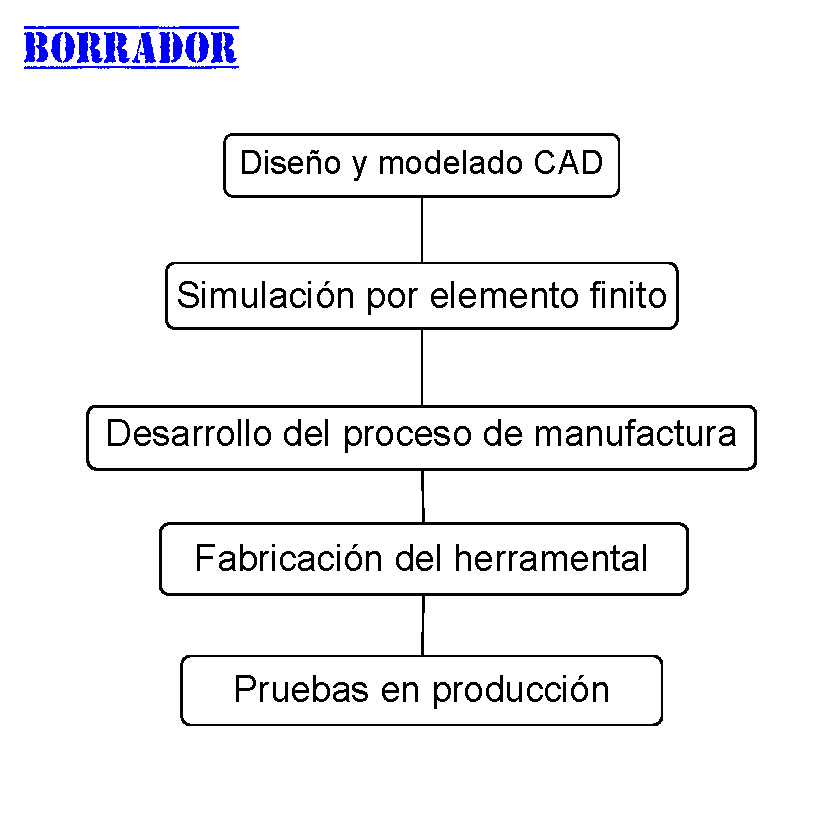
\includegraphics[width=0.75\textwidth]{src/ch3/diagrama_metodologia.pdf}
\captionof{figure}{Metodología del proyecto}
\label{fig:diagrama_metodologia}
\end{center}

\section{Consulta de fuentes de información}

En esta etapa inicial del proyecto se consultaron diversas fuentes de información 
relacionadas con los procesos de manufactura, específicamente los procesos 
de formado de hojas metálicas y operaciones de troquelado. Se buscó también información 
referente a la simulación por elementos finitos de operaciones que involucran 
deformación plástica, con la finalidad de conocer los tipos de análisis y definir 
el más conveniente para el caso. \\

Se consultó información relativa al estado del arte en artículos y/o publicaciones, 
sobre procesos de formado de manera general y para operaciones de doblado similares a la 
de este proyecto, es decir, aquellas que involucran una deformación sucesiva en UO. 
Todo esto se buscó en las principales bases de datos de contenido científico tales 
como Springer, Thomson, Elsevier, Scielo, Redalyc, así como en las bibliotecas 
digitales de diversas universidades hispanas y anglosajonas que proporcionan una 
cantidad considerable de trabajos de tesis, además de una revisión general en 
Google Scholar, que refiere e indexa la mayor parte del contenido de carácter científico 
y/o académico.

\section{Caracterización del material}

La caracterización del material es una cuestión importante, puesto que permitió conocer 
las propiedades mecánicas de interés, que sirvieron posteriormente para definir los 
modelos de los materiales asignados en el software de simulación.\\

El material utilizado como materia prima para el proceso de formado es un acero AISI 1018, 
muy común en la industria del troquelado, y cuyas propiedades mecánicas elementales están 
bastante caracterizadas en diversos reportes y/o \textit{handbooks} de materiales, pero 
es conveniente tomar en cuenta que no todos los materiales son sometidos al mismo proceso 
de fabricación y/o tratamientos, de modo que la caracterización en este caso servirá 
para validar esas propiedades, y además, obtener una curva de esfuerzo-deformación en la 
zona plástica.

\subsection{Ensayo de tensión uniaxial}

Cuando se requiere conocer las propiedades mecánicas de un material en ingeniería, se utilizan ensayos 
normalizados. En este caso se hace necesario obtener la curva esfuerzo-deformación del 
acero AISI 1018, misma que se utiliza como dato de entrada para la definición del material 
en el software de simulación utilizado. Para obtener el comportamiento esfuerzo-deformación 
de un metal se utiliza un ensayo de tensión uniaxial descrito en la norma ASTM-E8. ~\cite{ASTME8} \\

Se ensayaron cinco probetas planas, con las dimensiones descritas en la norma ATSM-E8, en una 
máquina de tensión MTS, obteniéndose los datos agrupados en la figura \ref{fig:tensile_test_all} para 
cada una de las probetas.\\

\begin{center}
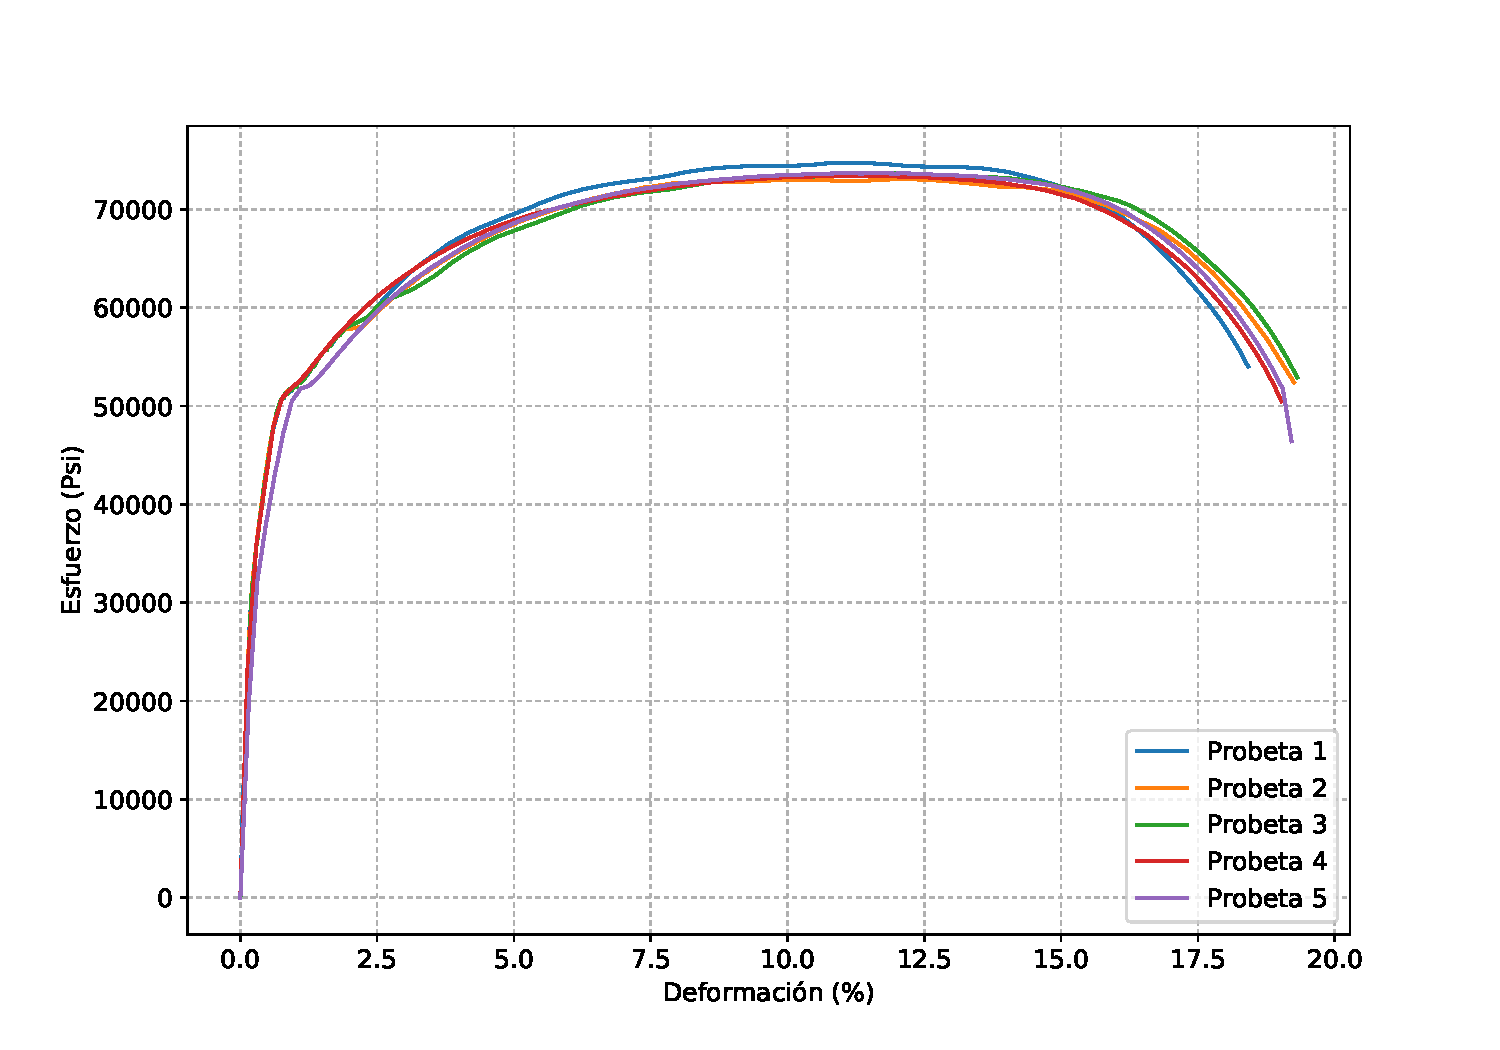
\includegraphics[width=0.7\textwidth]{src/ch3/tensile_test_all.pdf}
\captionof{figure}{Curvas de esfuerzo-deformación de las probetas ensayadas}
\label{fig:tensile_test_all}
\end{center}

Con los datos de las curvas de \ref{fig:tensile_test_all} se calculó un promedio de la relación esfuerzo-deformación, 
y se obtuvo una curva de esfuerzo-deformación promedio mostrada en la figura \ref{fig:material_curve}, 
en la cual se muestra, además, la curva esfuerzo-deformación verdadera calculada mediante las ecuaciones 
\ref{eq:true_stress} y \ref{eq:true_strain}.

\begin{center}
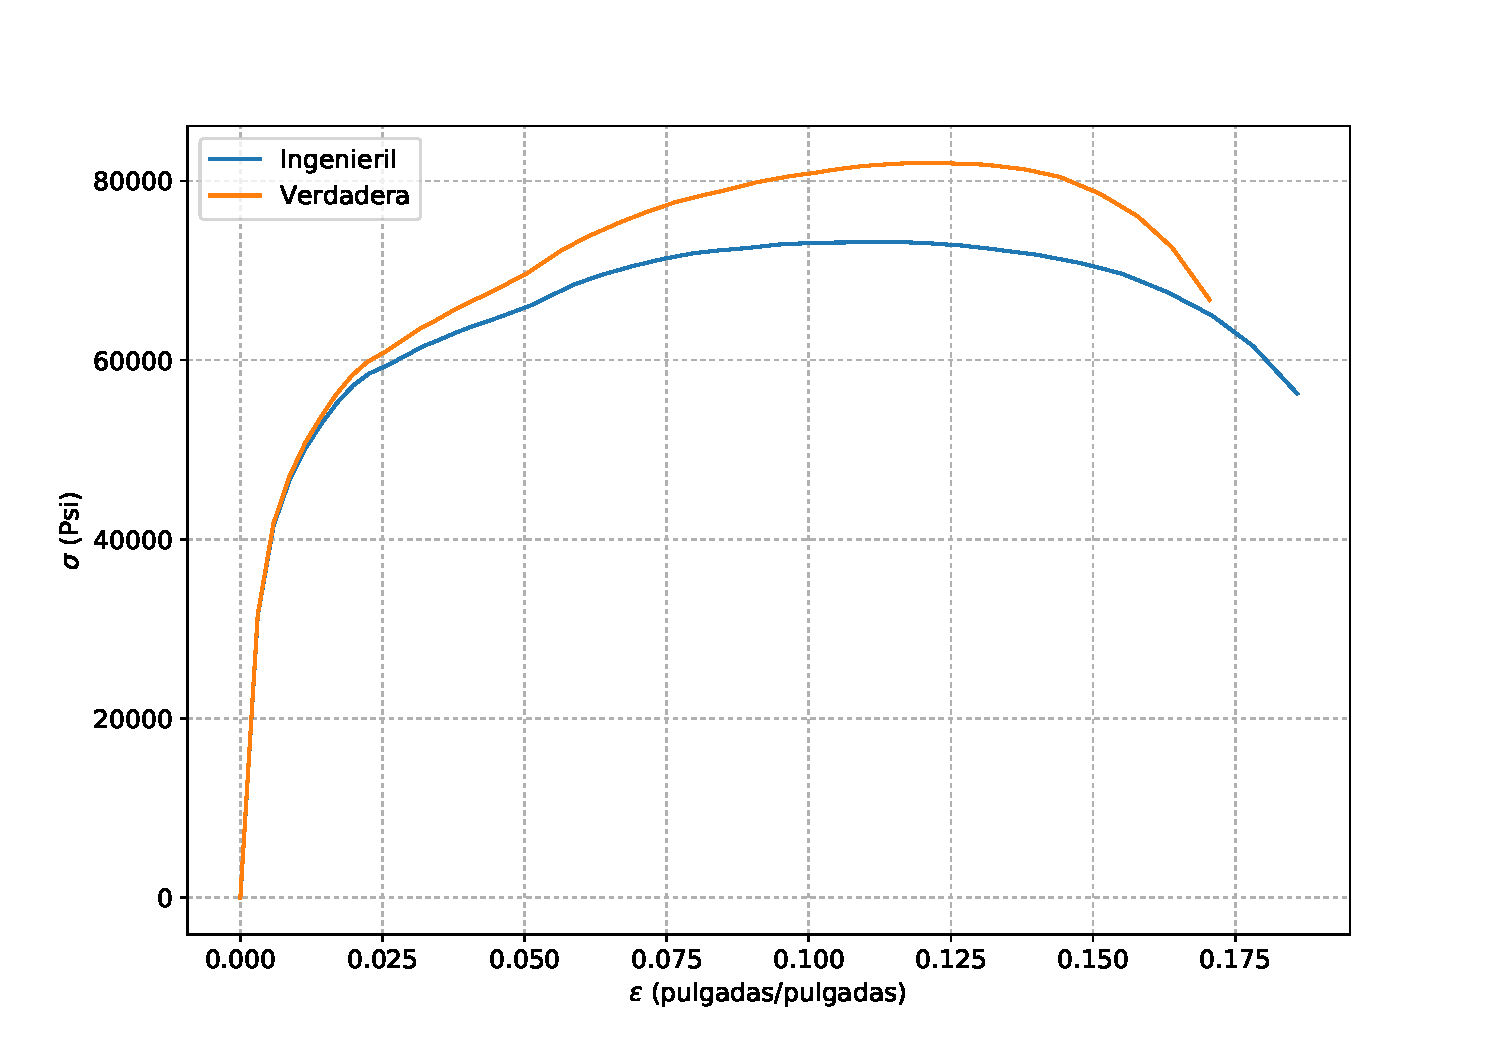
\includegraphics[width=0.7\textwidth]{src/ch3/material_curve.pdf}
\captionof{figure}{Curvas de esfuerzo-deformación, ingenieril y verdadera, del acero AISI 1018}
\label{fig:material_curve}
\end{center}

\section{Análisis por elementos finitos}

Como se describió en la sección \ref{subsec:implementacion-fem}, el análisis por elementos 
finitos en problemas de ingeniería es un proceso iterativo, en el que normalmente hay que ajustar 
algunos parámetros e ir revisando que los resultados obtenidos sean, al menos en principio, 
coherentes o se encuentren dentro de un rango esperado. \\

En el esquema mostrado en la figura \ref{fig:fem_diagram} se observa una metodología generalizada 
para un análisis por elementos finitos, partiendo desde el planteamiento de las 
ecuaciones diferenciales que gobiernan el problema. Cuando se utiliza un software 
de simulación, estos normalmente incorporan un entorno integrado que 
proporciona y facilita el desarrollo de un modelo de elementos finitos a partir 
de las geometrías involucradas, debido a esto, el proceso para el análisis por elementos 
finitos involucra algunas cuestiones como las que se muestran en el diagrama de 
la figura \ref{fig:metodologia_analisis_fem}, el cual sería más acorde con 
el proceso de análisis realizado en este caso.

\begin{center}
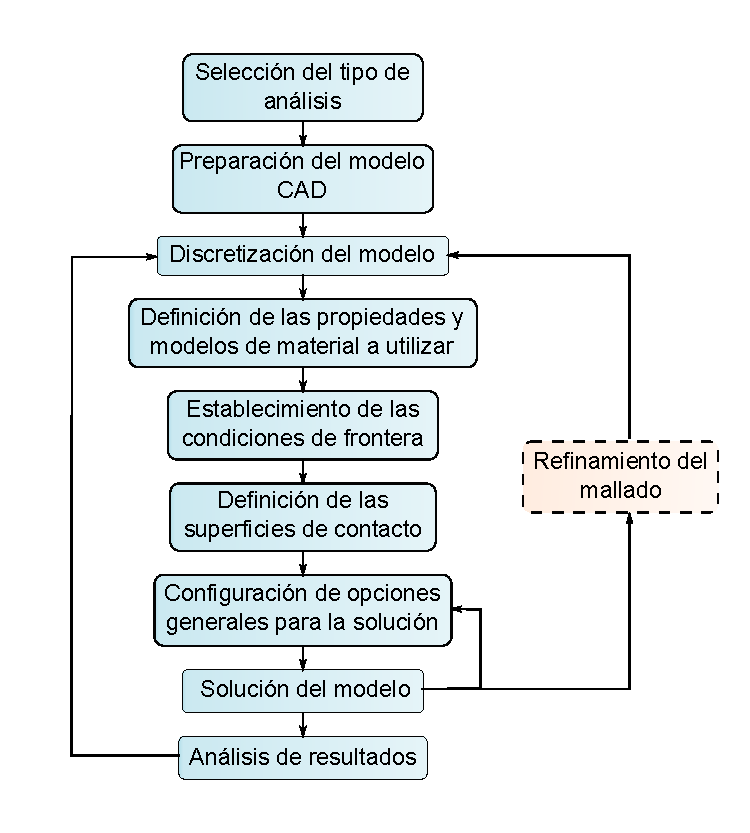
\includegraphics[width=0.75\textwidth]{src/ch3/metodologia_analisis_fem.pdf}
\captionof{figure}{Metodología para el análisis por elemento finito}
\label{fig:metodologia_analisis_fem}
\end{center}

\subsection{El proceso a simular}

En el capítulo \ref{ch:marco_de_referencia} se ha descrito someramente el proceso de formado que se requiere 
simular. Ahora, en lo subsiguiente, se detallan en mayor grado las características 
relativas al proceso, materiales utilizados y condiciones de operación que influyen en este. \\

El tubo interior mostrado en la figura \ref{fig:ti_rb131} se utiliza en un buje como 
el mostrado en la figura \ref{fig:buje_rb131}, el cual forma parte de un sistema de muelles 
parabólicas.

\begin{figure}[H]
\centering
\begin{subfigure}[t]{0.35\textwidth}
\centering
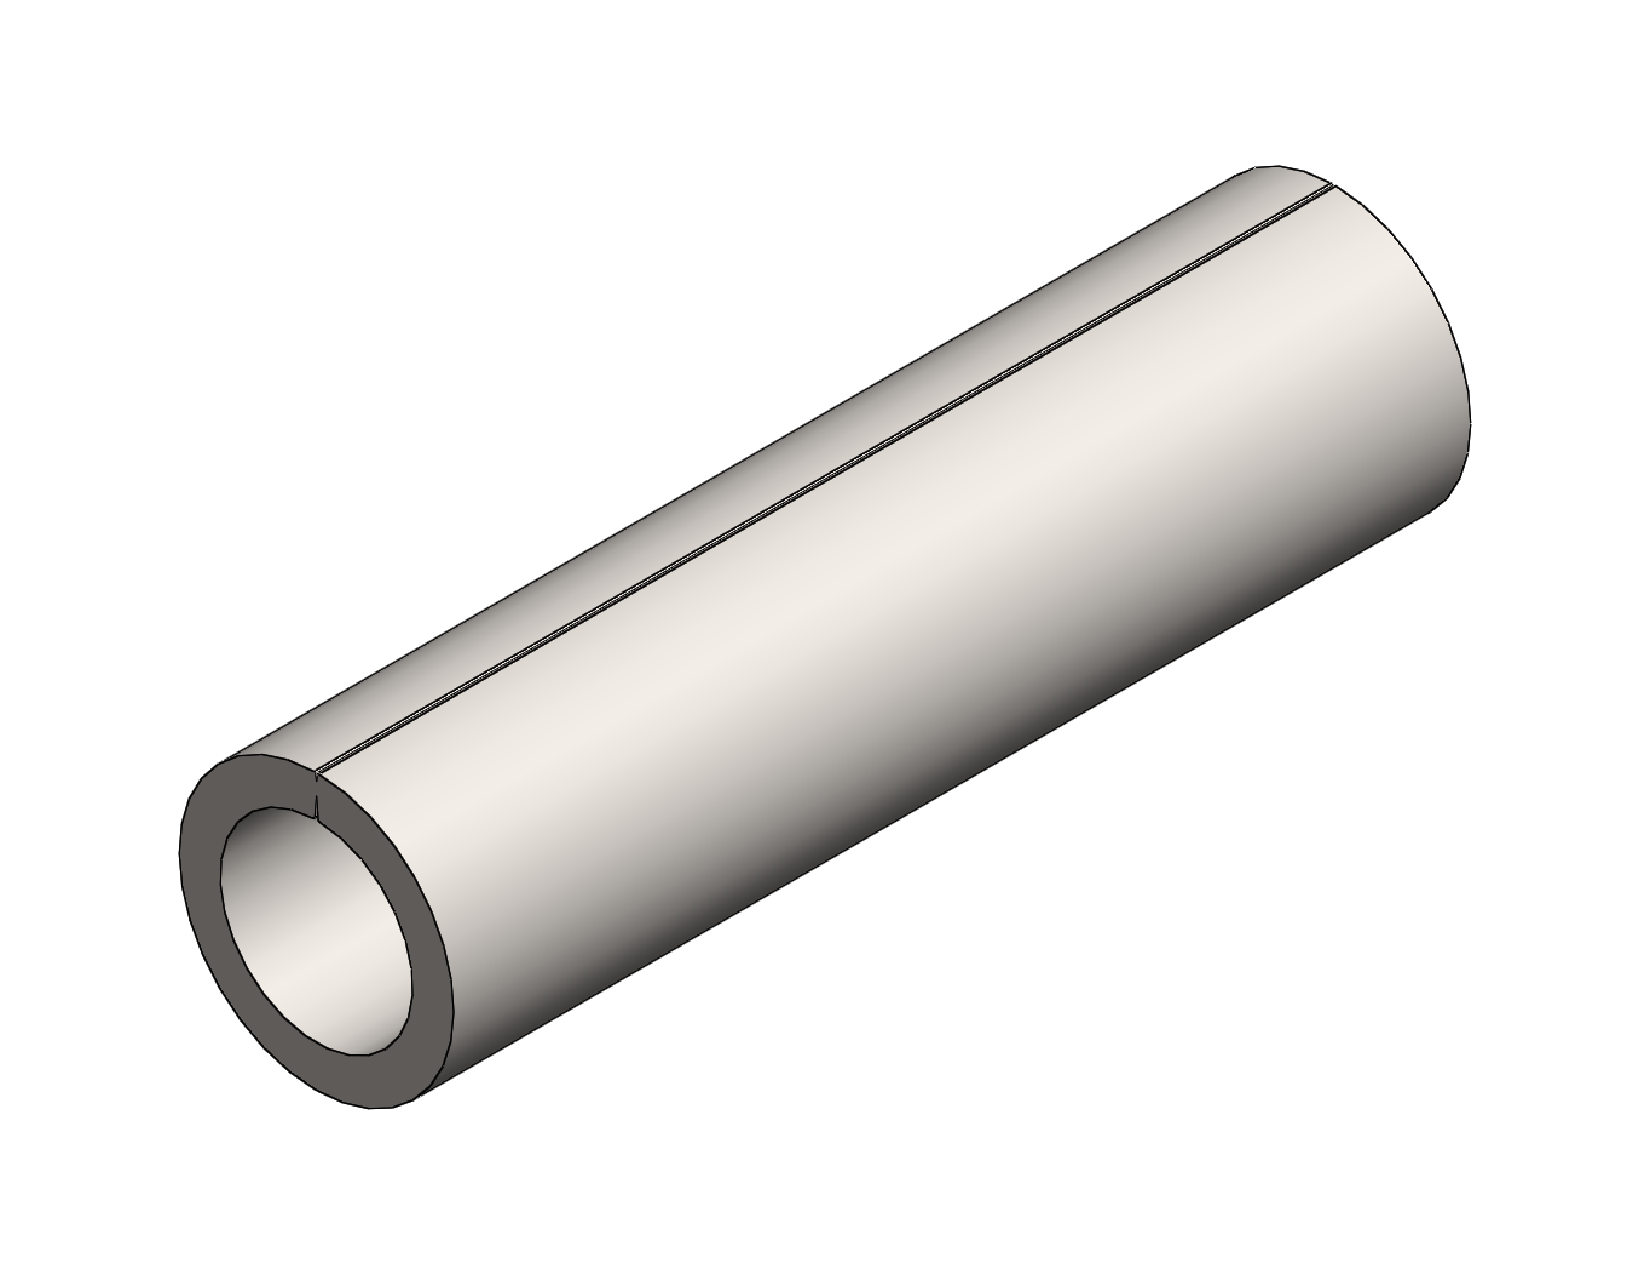
\includegraphics[width=\textwidth]{src/ch3/ti_rb131.pdf}
\caption{}
\label{fig:ti_rb131}
\end{subfigure}
~  
\begin{subfigure}[t]{0.35\textwidth}
\centering
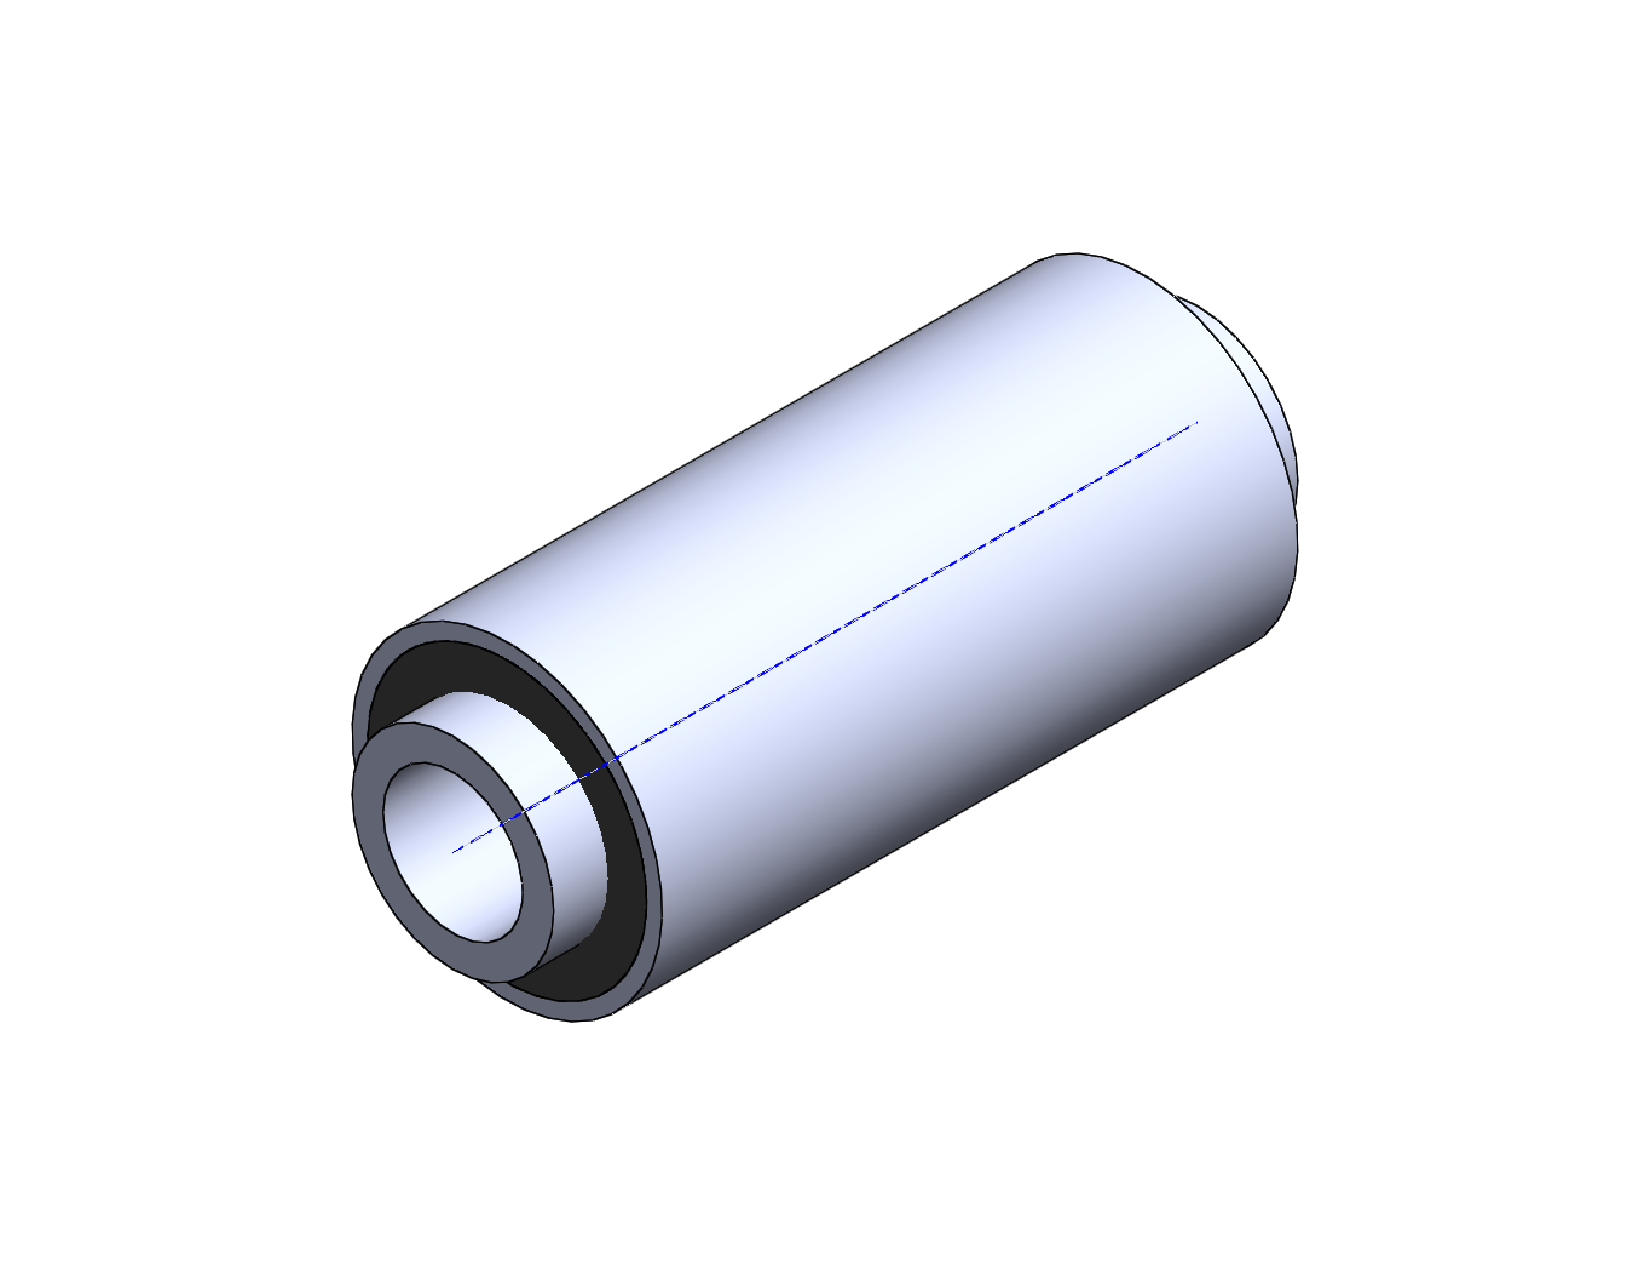
\includegraphics[width=\textwidth]{src/ch3/buje_rb131.pdf}
\caption{}
\label{fig:buje_rb131}
\end{subfigure}
\caption{a) Modelo CAD del tubo interior manufacturado por estampado b) Modelo CAD del buje RB-131}
\end{figure}


Para fabricar el tubo interior \ref{fig:ti_rb131} se utiliza un troquel compuesto o semiprogresivo 
de dos etapas, a saber: un doblado en U y un cerrado o doblado en O, mismo cuyo modelo CAD se muestra 
en la figura \ref{fig:troquel}. El troquel tiene como materia de entrada una placa metálica 
(\textit{blank}) rectangular de acero AISI 1018, con un largo de 3 in y un acho de 2.125 in, 
con un espesor de 0.12 in (ver figura \ref{fig:blank_inicial}). El \textif{blank} tiene además 
dos chaflanes en la dirección axial, sobre una de las caras, mismos que sirven para permitir un 
cierre de tubo adecuado.

% \begin{center}
% 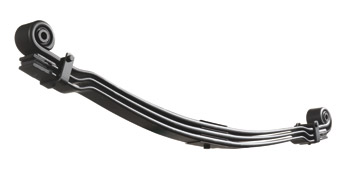
\includegraphics[scale=0.65]{src/ch3/muelle_parabolica.jpg}
% \captionof{figure}{Muelle parabólica}
% \label{fig:muelle_parabolica}
% \end{center}


\begin{center}
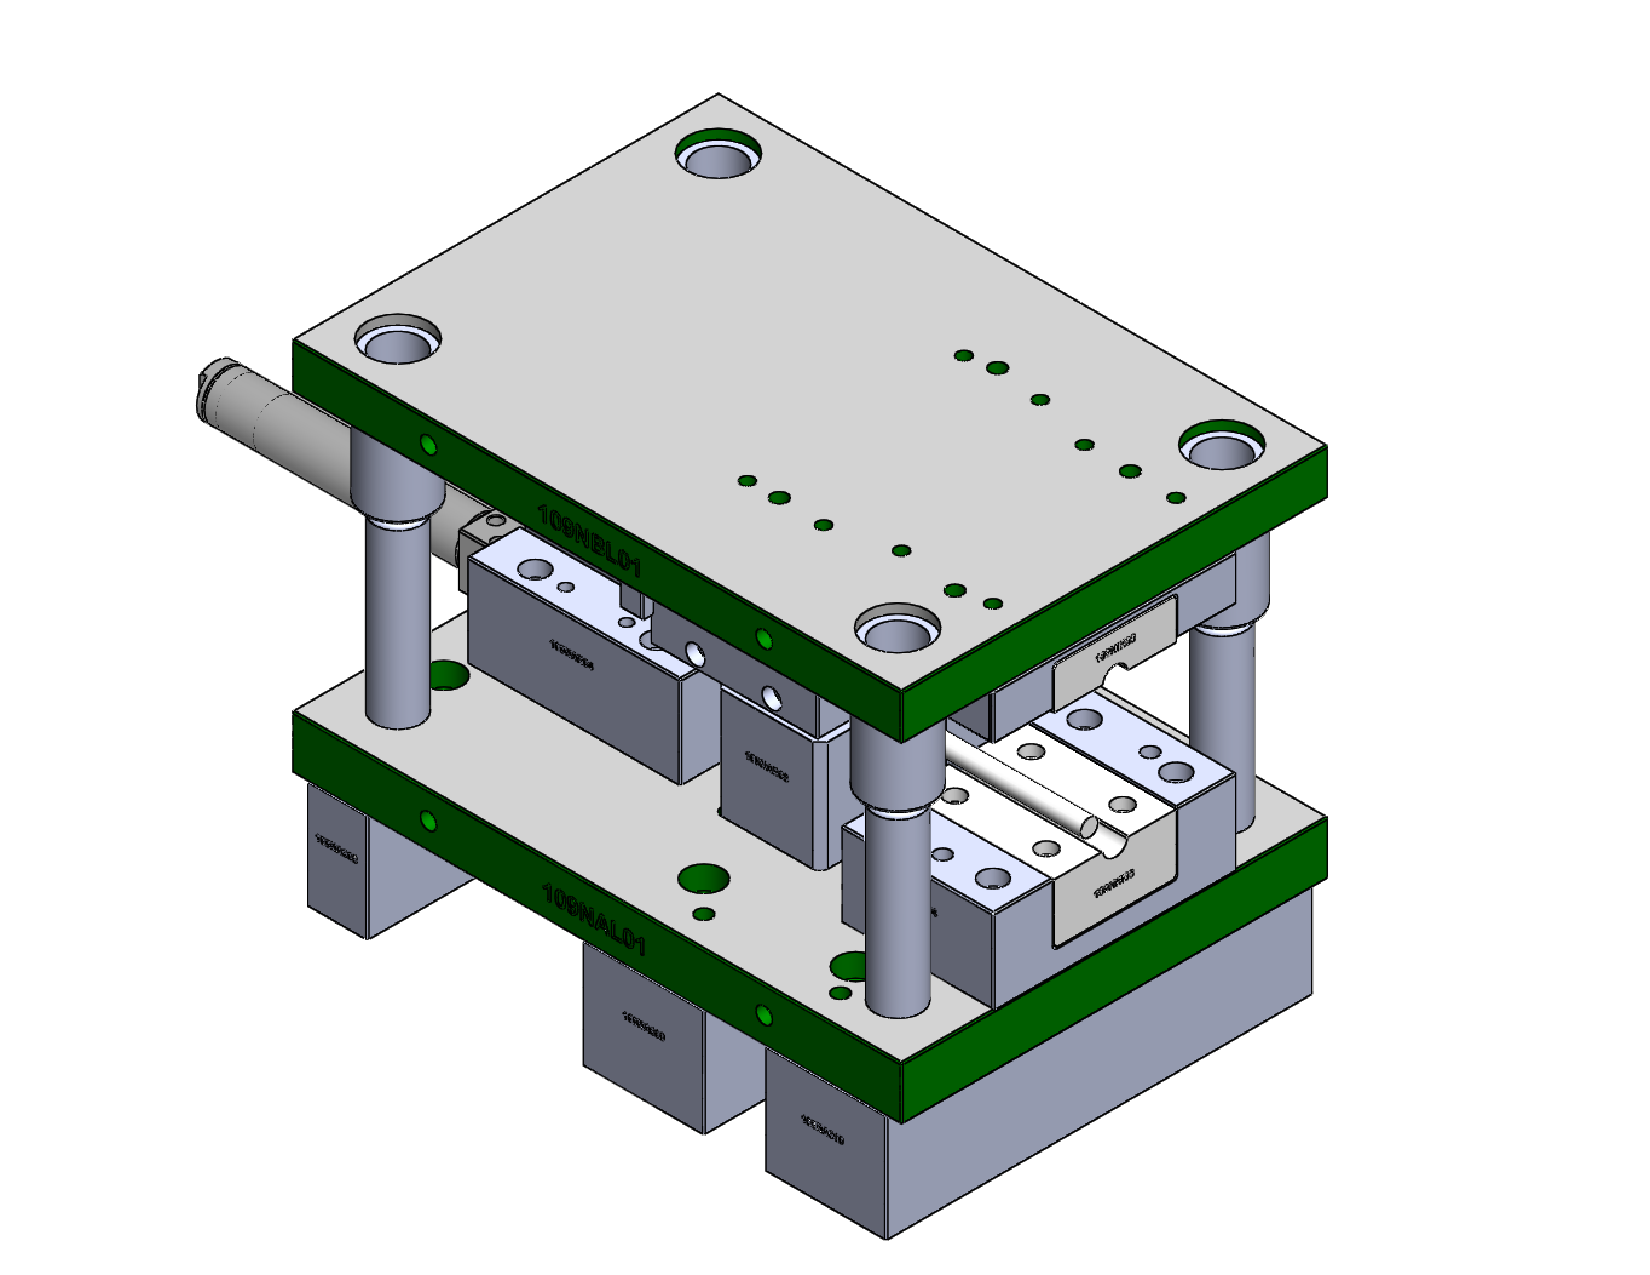
\includegraphics[scale=0.4]{src/ch3/troquel.pdf}
\captionof{figure}{Vista completa del troquel}
\label{fig:troquel}
\end{center}

% \begin{figure}[H]
% \centering
% \begin{subfigure}[t]{0.45\textwidth}
%     \centering
%     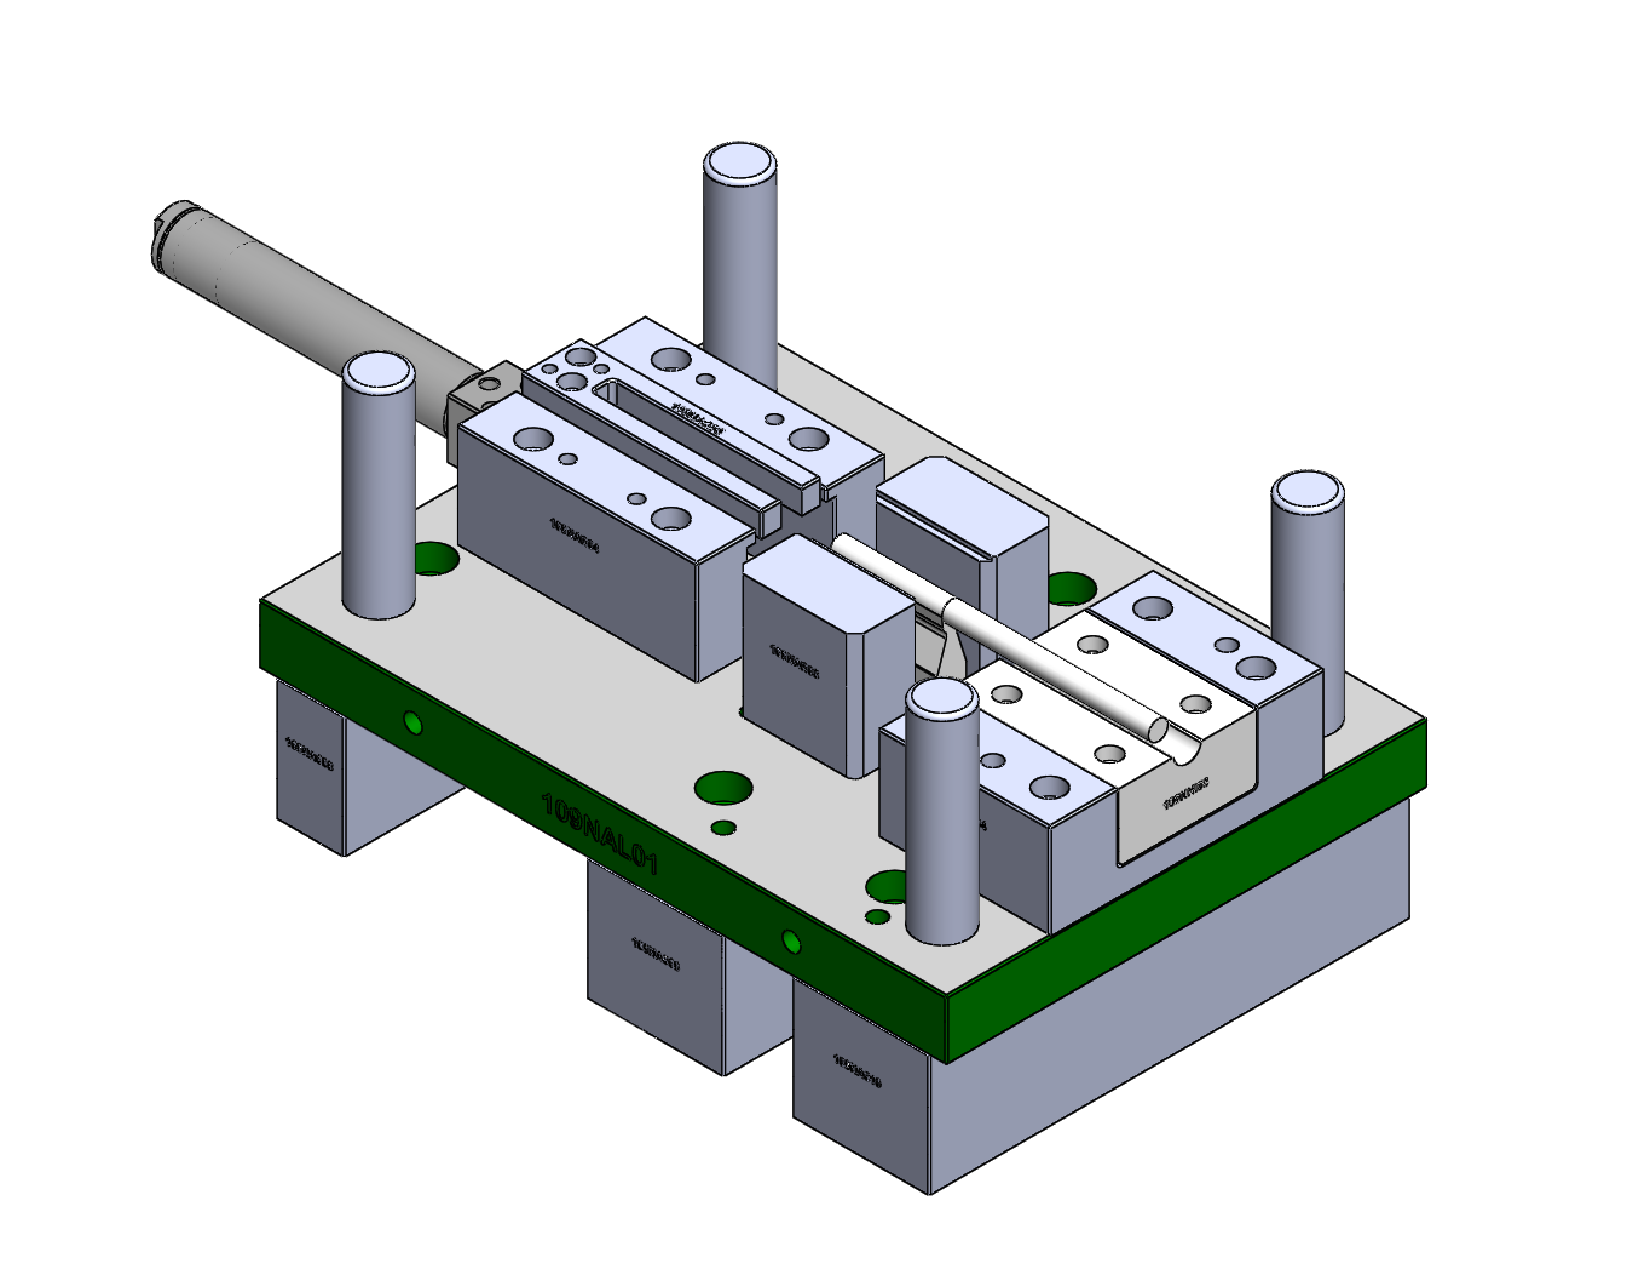
\includegraphics[width=\textwidth]{src/ch3/troquel_vista_inferior.pdf}
%     \caption{}
%     \label{fig:troquel_vista_inferior}
% \end{subfigure}
% ~ 
% \begin{subfigure}[t]{0.45\textwidth}
%     \centering
%     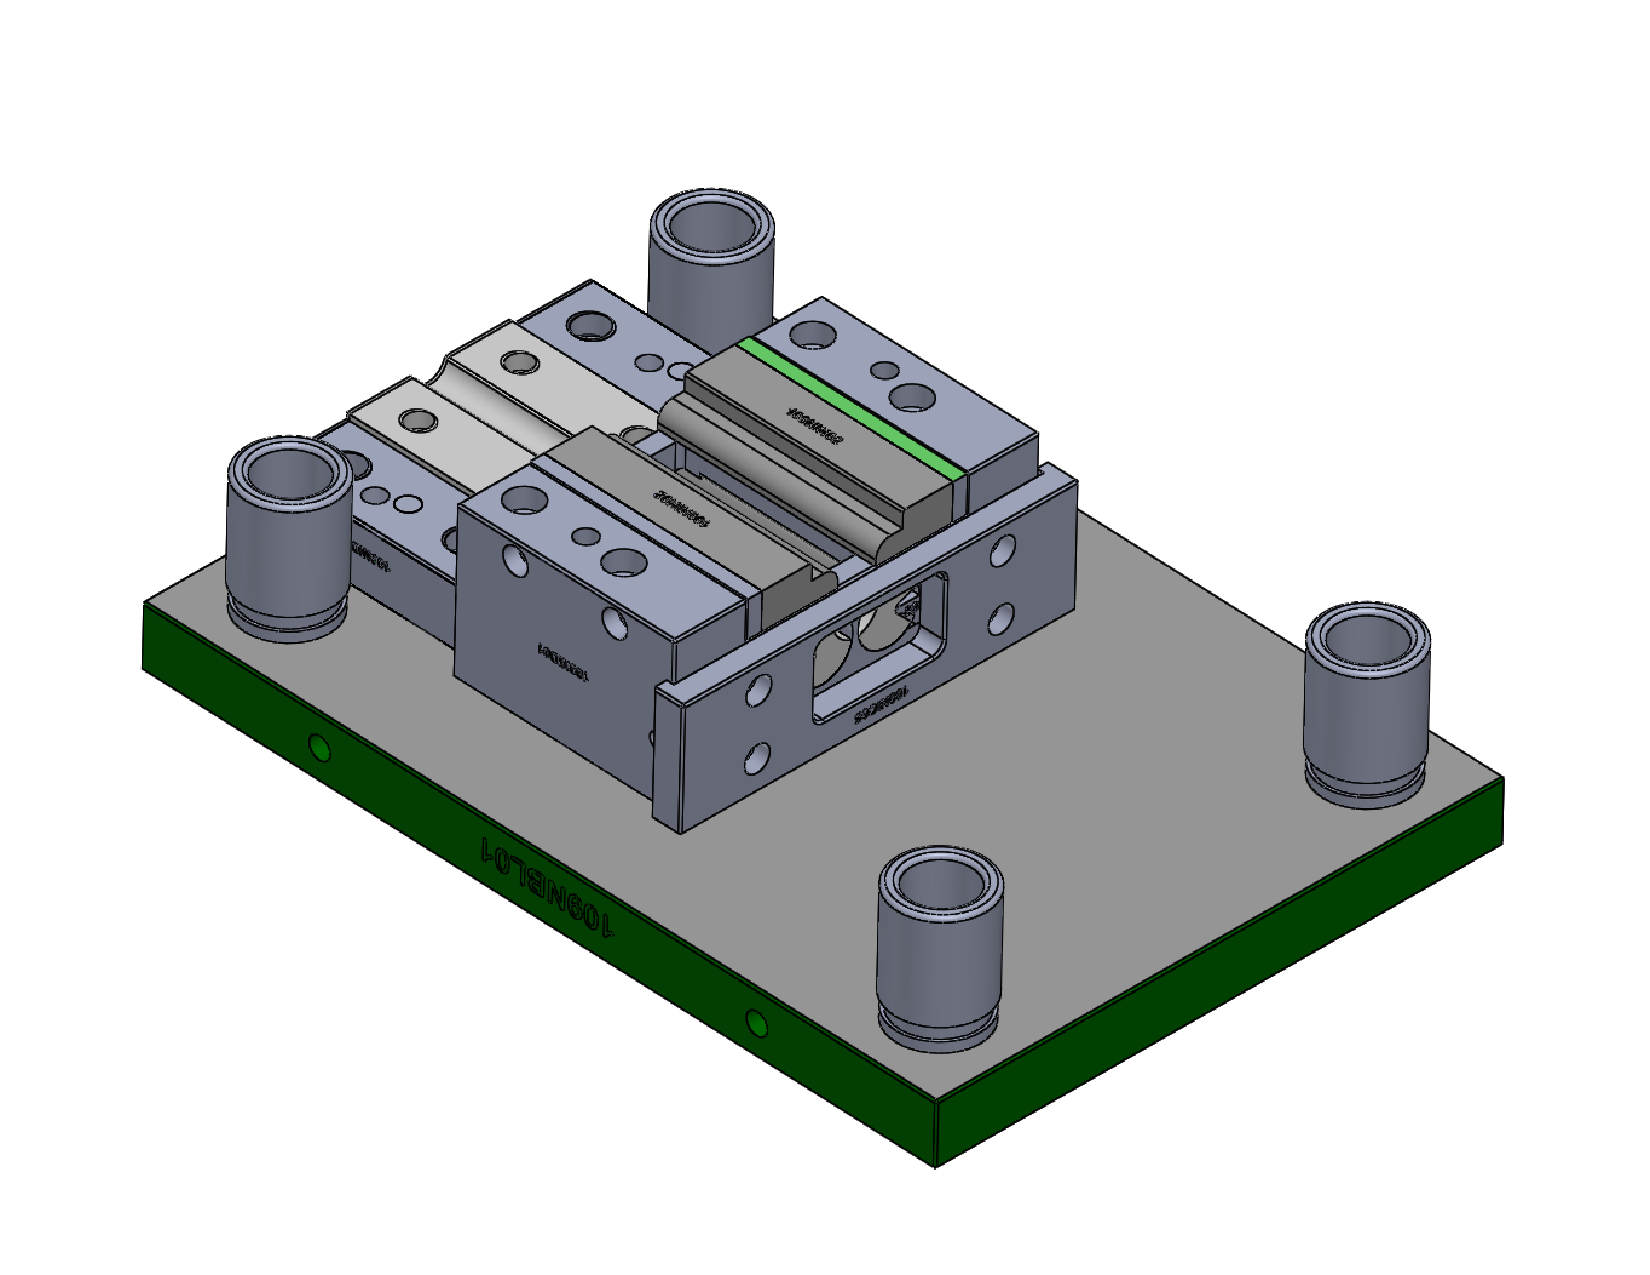
\includegraphics[width=\textwidth]{src/ch3/troquel_vista_superior.pdf}
%     \caption{}
%     \label{fig:troquel_vista_superior}
% \end{subfigure}
% \caption{Partes a) inferior y b) superior del troquel}
% \end{figure}


\begin{center}
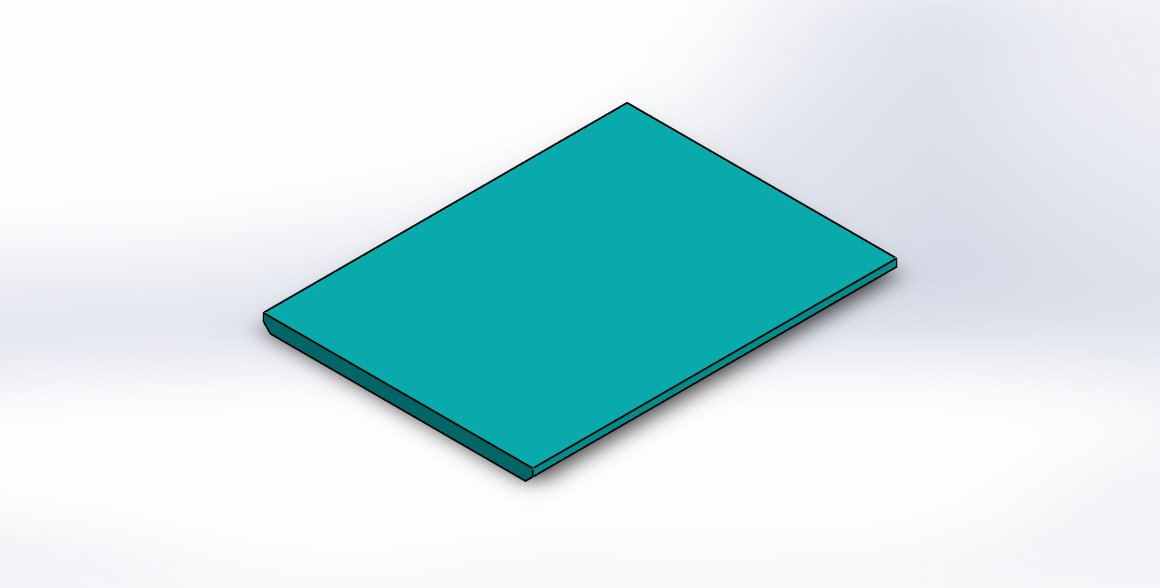
\includegraphics[width=0.6\textwidth]{src/ch3/blank.jpg}
\captionof{figure}{Pieza de trabajo de entrada}
\label{fig:blank_inicial}
\end{center}

\subsection{Consideraciones generales}\label{sec:consideraciones-generales}

En la sección anterior se describe la pieza de trabajo utilizada y las características del herramental 
utilizado para el proceso de formado, sin embargo para llevar a cabo la simulación por elementos 
finitos es necesario hacer algunas consideraciones, mismas que se describen a continuación.\\

Siguiendo la lógica del proceso real, la simulación se dividió en dos etapas: el preformado en U y 
el cerrado del tubo. Esto permite realizar dos análisis de menor costo computacional que uno entero, 
además de evitar las complicaciones inherentes al tiempo de vida de los contactos y el correcto 
posicionamiento de los formadores para cada caso.\\

Para lo anterior se tuvieron dos ensambles correspondientes al primer (ver figura \ref{fig:assembly_01}) y 
segundo paso (ver figura \ref{fig:assembly_02}) del troquel. En el primer paso se realizó 
un análisis dinámico-explícito ordinario, definiendo los modelos de material, la discretización y 
la definición de contactos. En el segundo paso se realizó un análisis de tipo \textit{full restart} o 
\textit{análisis de reinicio}, que básicamente consiste en crear una base de datos de análisis a 
partir de otro realizado, importanto la geometría deformada de la pieza de trabajo, así como toda 
la información referente a la definición de materiales, partes, contactos, y distribución de esfuerzos. 
En la sección \ref{sec:initial-stress} se describe de manera detallada este proceso. \\

La figura \ref{fig:assembly_01} muestra las geometrías que componen el ensamble del primer paso, 
que consta de un formador inferior que funge como un tipo de \textit{matriz} y es sobre la cual 
se dobla el material, dos formadores superiores que ejecutan el doblado en U, y dos levas 
que tienen la función de realizar un doblado más pronunciado a los extremos de la pieza de 
trabajo y que permite un cierre más adecuado cuando se realiza el último paso del troquel.
De igual manera, en la figura \ref{fig:assembly_02} se muestra el ensamble correspondiente 
al segundo paso del troquel, que consta de un formador superior y formador inferior que contienen 
la misma forma negativa (un semicírculo), con la diferencia evidente que el primero es el que ejerce 
el trabajo de formado aplicado sobre la pieza, adémás se tiene un perno formador que permite 
un cierre adecuado del tubo, conservando las especificaciones geométricas para el diámetro interior.

\begin{center}
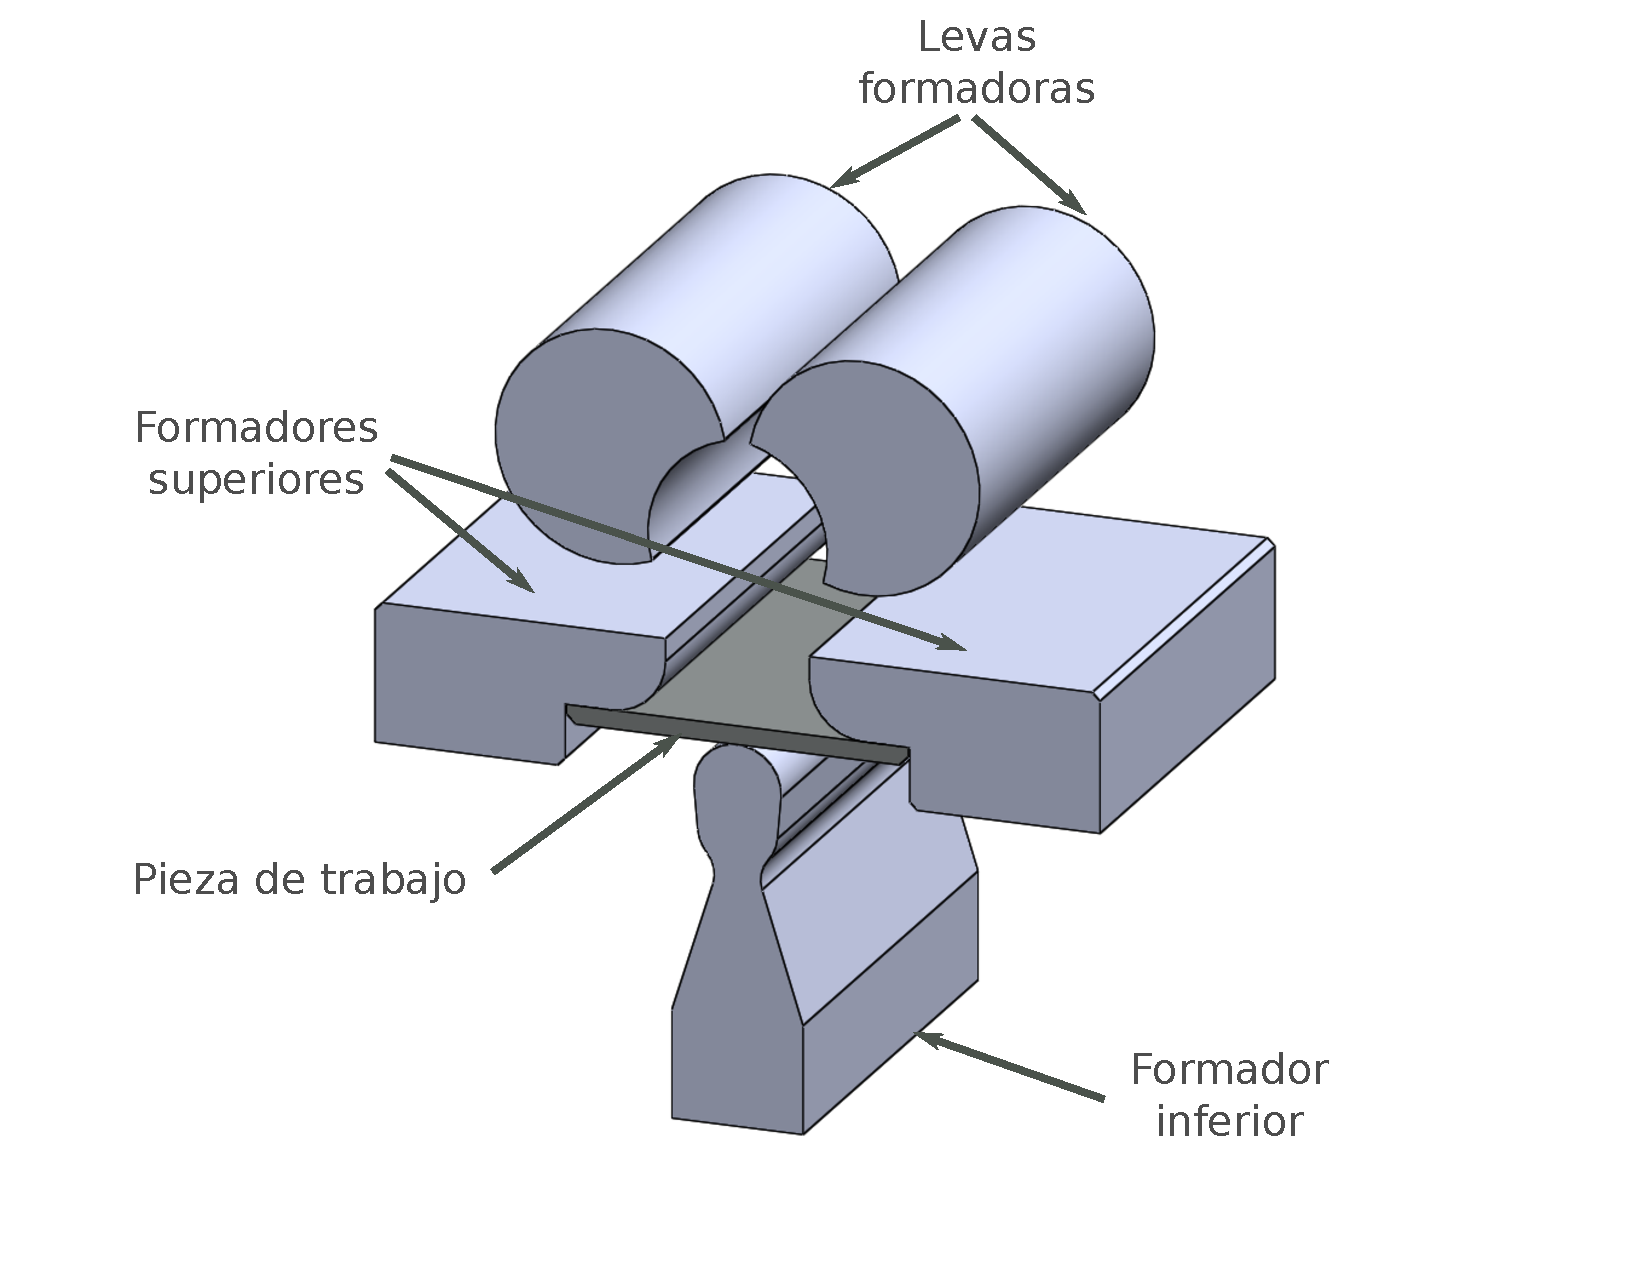
\includegraphics[width=0.6\textwidth]{src/ch3/assembly_01.pdf}
\captionof{figure}{Ensamble primera etapa}
\label{fig:assembly_01}
\end{center}

\begin{center}
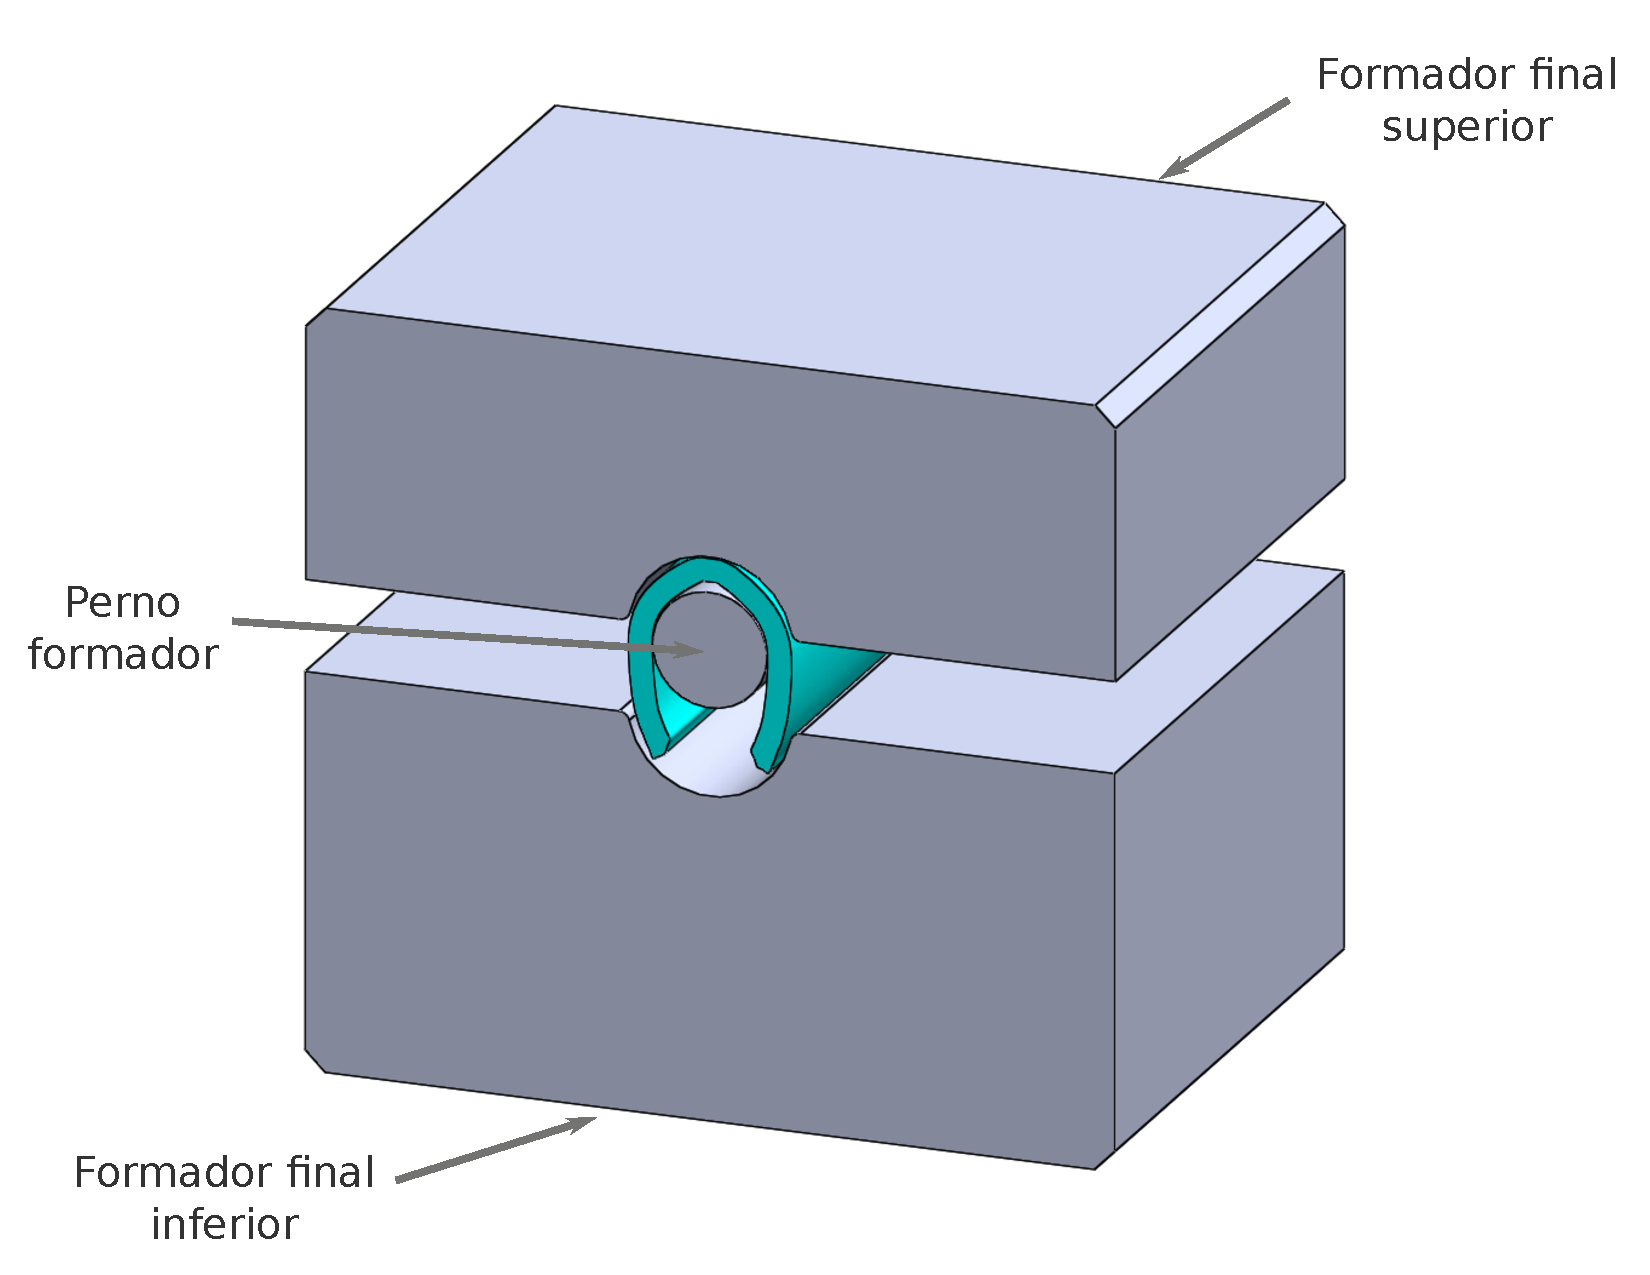
\includegraphics[width=0.6\textwidth]{src/ch3/assembly_02.pdf}
\captionof{figure}{Ensamble segunda etapa}
\label{fig:assembly_02}
\end{center}

\subsection{Modelo constitutivo}

Para la pieza de trabajo se utilizó un modelo de tipo \textit{Piecewise Linear Plasticity}, 
el cual es un modelo multilineal que permite utilizar una curva esfuerzo-deformación y la 
dependencia de la tasa de deformación como datos de entrada para definir el comportamiento 
plástico del material. Para cuantificar la tasa de deformación este modelo utiliza la 
relación de Cowper-Symonds mostrada en la ecuación \ref{eq:cowper_symonds}.\\

\begin{equation} \label{eq:cowper_symonds}
\sigma_{y}\left( \varepsilon _{eff}^{P},\dot{\varepsilon }_{eff}^{P} \right) = 
{{\sigma }_{y}}\left( \varepsilon _{eff}^{P} \right)\left[ 1+{{\left( \frac{\dot{\varepsilon }_{eff}^{P}}{C} \right)}^{\frac{1}{P}}} \right]
\end{equation}

La curva esfuerzo-deformación ingresada en el software de simulación fue la obtenida 
de forma experimental, con algunas modificaciones a saber: se tomaron solamente 7 puntos 
de la curva original linealmente equiespaciados, se calculó el esfuerzo y deformación verdadera 
mediante las ecuaciones descritas en la sección \ref{subsec:true_strain_stress}, posteriormente 
a partir de la deformación verdadera se obtuvo la deformación plástica mediante la 
ecuación \ref{eq:plastic_strain}, mismas que se agrupan en la tabla \ref{tab:strain_stress_conversion}.
La curva resultante y que se ingresó en el softaware se muestra en la figura \ref{fig:ls_dyna_material_curve}. \\

Para definir completamente el modelo es necesario asignar las propiedades mecánicas elementales 
como el módulo elástico, la relación de Poisson y la densidad. Además, se debe asignar 
la resistencia a la fluencia y las constantes C y P utilizadas en la ecuación de Cowper-Symonds.
Estas propiedades utilizadas se muestran en la tabla \ref{tab:material_properties}. \\

% Tabla de propiedades
\begin{table}[h]
\centering
\caption{Propiedades del acero AISI 1018}
\label{tab:steel_properties}
\begin{tabular}{p{4cm} p{4cm}} \hline
Propiedad & Magnitud (unidades) \\
\hline
Módulo elástico & 29 000 (ksi) \\
Densidad & 0.00073 (lbf s$^2$/in$^4$) \\
Esfuerzo de fluencia & 52 000 (psi) \\
Coeficiente de Poisson & 0.3 \\
C & 40 (s$^{-1}$) \\
P & 5 \\
\hline
\end{tabular}
\label{tab:material_properties}
\end{table}

En los componentes del troquel se utilizó un modelo rígido, para el cual sólo es necesario 
especificar las propiedades elásticas. Los componentes rígidos, normalmente, permiten la 
aplicación de condiciones de desplazamiento utilizando el identificador o ID de la parte, además 
se pueden asignar propiedades de inercia o velocidades iniciales. En este caso, no se 
especificaron propiedades adicionales, lo cual implica que el software de simulación calcule automáticamente 
las propiedades inerciales basadas en el modelo de elemento finito. \\

Para crear los materiales de cada uno de los componentes se utilizó un pequeño \textit{script}, el 
cual se anexa en \ref{sec:definicion-materiales}

% Tabla de propiedades plásticas

\begin{table}[h]
\centering
\caption{Conversión de esfuerzos y deformaciones}
\label{tab:strain_stress_conversion}
\begin{tabular}{p{2.5cm} p{2.5cm} p{2.5cm} p{2.5cm} p{2.5cm}} \hline
{\bf $\varepsilon_{nom}$ & $\sigma_{nom}$ (psi) & $\varepsilon_t$ & $\sigma_t$ (psi) & $\varepsilon_{pl}$ } \\
\hline
0.0084 & 51376.41 & 0.0084 & 51808.49 & 0.0000 \\
0.0224 & 59624.27 & 0.0221 & 60957.47 & 0.0200 \\
0.0418 & 67059.05 & 0.0409 & 69858.77 & 0.0385 \\
0.0607 & 70769.55 & 0.0589 & 75063.85 & 0.0563 \\
0.0846 & 72814.73 & 0.0812 & 78971.94 & 0.0785 \\
0.1287 & 72924.09 & 0.1210 & 82305.77 & 0.1182 \\
0.1554 & 70462.94 & 0.1444 & 81412.18 & 0.1416 \\
\hline
\end{tabular}
\label{tab:stress_strain_curve}
\end{table}


\begin{center}
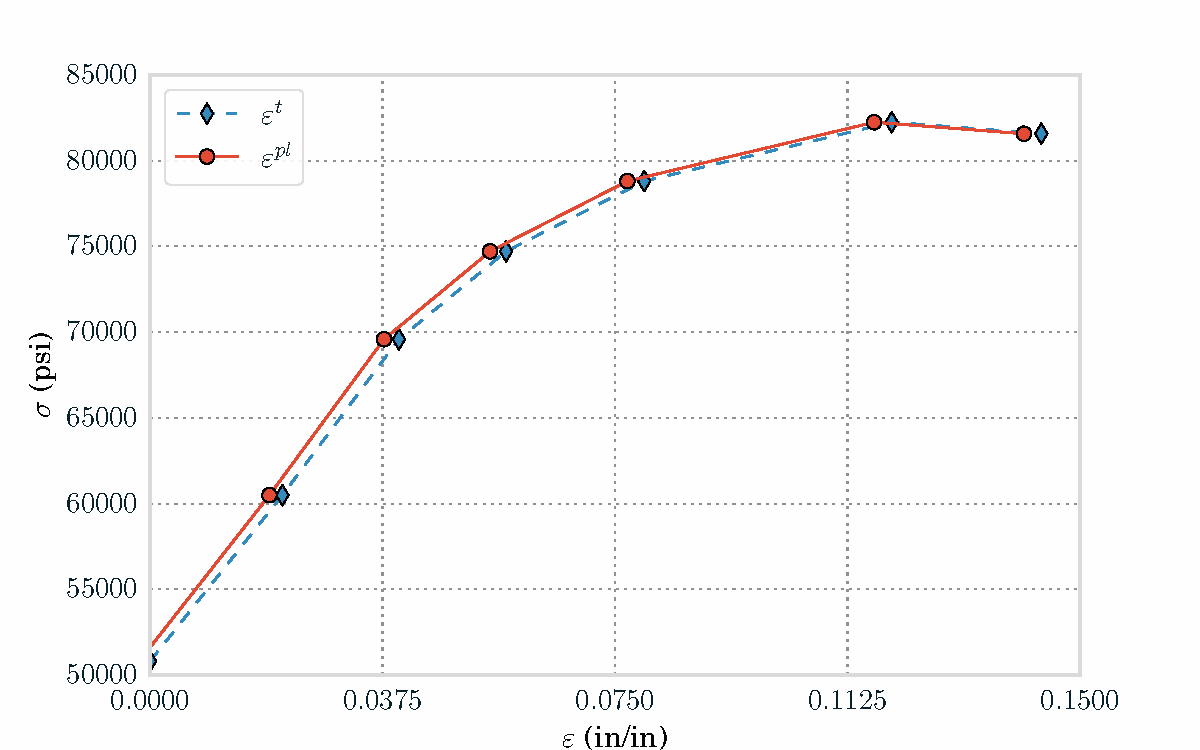
\includegraphics[scale=0.6]{src/ch3/ls_dyna_material_curve.pdf}
\captionof{figure}{Curva esfuerzo-deformación ingresada en ANSYS/LS-DYNA}
\label{fig:ls_dyna_material_curve}
\end{center}

\subsection{Análisis bidimensional}

\subsubsection{Preparación de la geometría}

Para cada uno de los ensambles correspondientes a cada paso se importó un archivo de tipo parasólido 
que fue exportado desde el software de CAD utilizado para modelar y diseñar el herramental. Se utilizó 
un tipo parasólido debido a su extensa interoperabilidad con diversos paquetes de CAD/CAE. ~\cite{parasolid-reference} \\

Normalmente un archivo parasólido guarda información utilizando el metro como unidad fundamental 
de longitud, aún cuando en el software CAD se hayan diseñado las piezas en otras unidades. 
Así, en este caso, fue necesario escalar el modelo importado para convertir los metros a pulgadas 
y trabajar en el sistema inglés, esto mediante las herramientas de modelado proporcionadas por 
ANSYS\CR. \\

Del modelo CAD importado el softaware de simulación crea entidades geométricas de volumen, áreas, 
líneas y \textit{keypoints}. Pero para el análisis bidimensional sólo se necesitaron las áreas 
correspondientes a la vista frontal del modelo, por tanto se procedió a eliminar las todas las entidades 
de volumen y área, para poder borrar las lineas correspondientes a la dirección axial del modelo.
Quedando solamente entidades de línea correspondientes a la sección transversal y creando  
a partir de estas nuevas áreas con las cuales se trabajó en el análisis de elementos finitos.


\subsubsection{Mallado}

En esta sección se describe el proceso de mallado para el análisis bidimensional realizado, 
mismo para el cual se asumió una condición de deformación plana. Es importante mencionar 
que durante esta sección cuando se hable de mallar geometrías se estará haciendo referencia 
implícita a áreas.\\

Se utilizó el elemento \texttt{PLANE162}, mismo cuyo esquema se muestra en la figura \ref{fig:plane162}, 
el cual es utilizado para el modelado 2D de estructuras sólidas, este elemento puede ser utilizado en 
análisis de deformación y esfuerzo plano y para análisis axisimétricos. El elemento es definido por 
cuatro nodos teniendo seis grados de libertad en cada uno de ellos: traslaciones, velocidades y 
aceleraciones en las direcciones \texttt{x} e \texttt{y}. Este elemento soporta la mayoría de los modelos 
de materiales utilizados en el formado de metales, tales como bilineal isotrópico y cinemático, plasticidad 
cinemática, Johnson-Cook, curva multilineal, entre otros. \\

El elemento \texttt{PLANE162} se usó con la opción de deformación plana y formulación lagrangiana, esto controlado 
desde los \textit{keyoption} al definir el tipo de elemento, seleccionando además la opción de \textit{full integration} 
para evitar los efectos de los modos de deformación derivados de la energía de Hourglass o de energía cero, los cuales 
deforman la malla en forma de zig zag e inducen esfuerzos elevados en las zonas deformadas.\\

\begin{center}
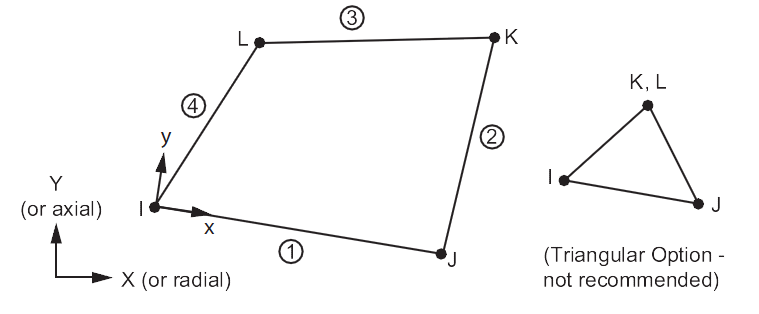
\includegraphics[width=0.65\textwidth]{src/ch3/plane162.png}
\captionof{figure}{Elemento \texttt{PLANE162}}
\label{fig:plane162}
\end{center}

El \textit{blank} se malló con elementos cuyo tamaño global fue de 0.03 in. Debido a los chaflanes del blank 
un mallado mapeado produce una malla bastante irregular, por ello se dividió el blank en 5 áreas, resultando 
en áreas correspondientes a polígonos regulares, que pudieron mallarse de forma más refinada, quedando una malla 
bastante regular y con elementos proporcionados como se observa en la figura \ref{fig:mesh_blank_2d}

\begin{center}
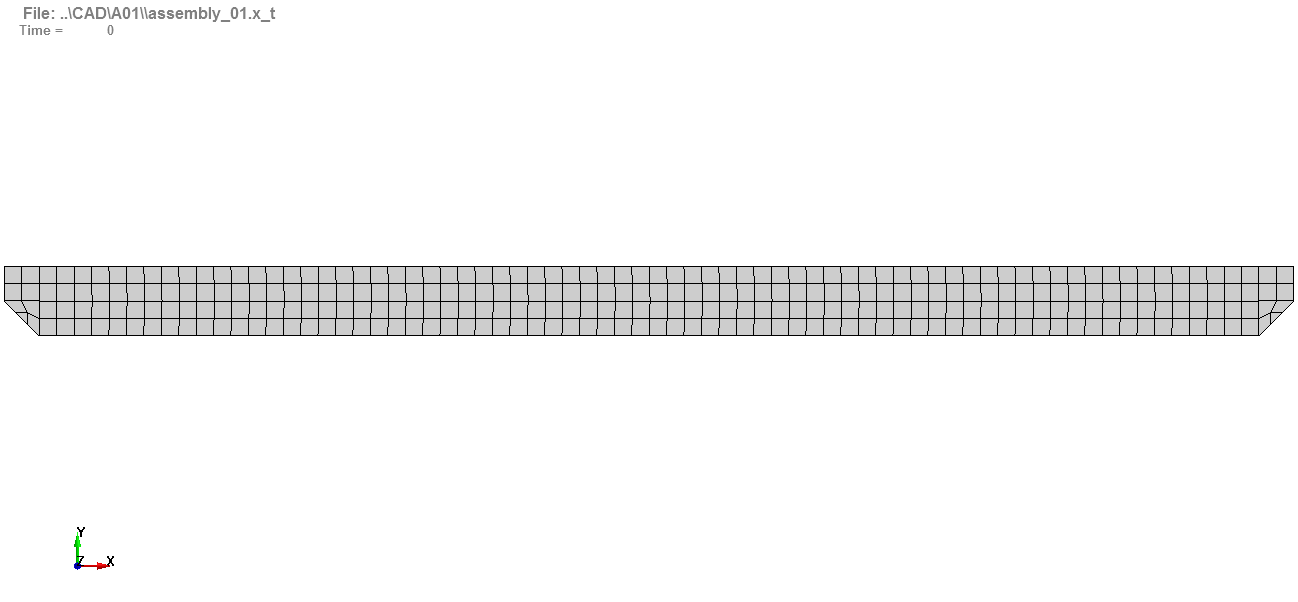
\includegraphics[width=0.55\textwidth]{src/ch3/mesh_blank_2d.png}
\captionof{figure}{Mallado del \textit{blank}}
\label{fig:mesh_blank_2d}
\end{center}

Para el mallado de los formadores, cada uno se dividió en dos regiones, una de las cuales está en contacto directo 
con el blank durante el proceso de formado. Así, para la región que está en contacto para cada caso, se asignó 
a las líneas un tamaño de elemento de 0.025 in, con la finalidad de tener regiones con una densidad de malla mayor 
que permitiese un adecuado comportamiento de los formadores. \\

Una densidad de malla mayor es importante y necesaria sobre todo en las partes agudas de las levas mostradas en 
las figuras \ref{fig:mesh_leva_izq_2d} y \ref{fig:mesh_leva_der_2d}, puesto que si se mallan de manera más burda 
se presentan problemas de contacto con la pieza de trabajo, resultando en deformaciones inusuales y daño sobre 
el material en formado.

\begin{center}
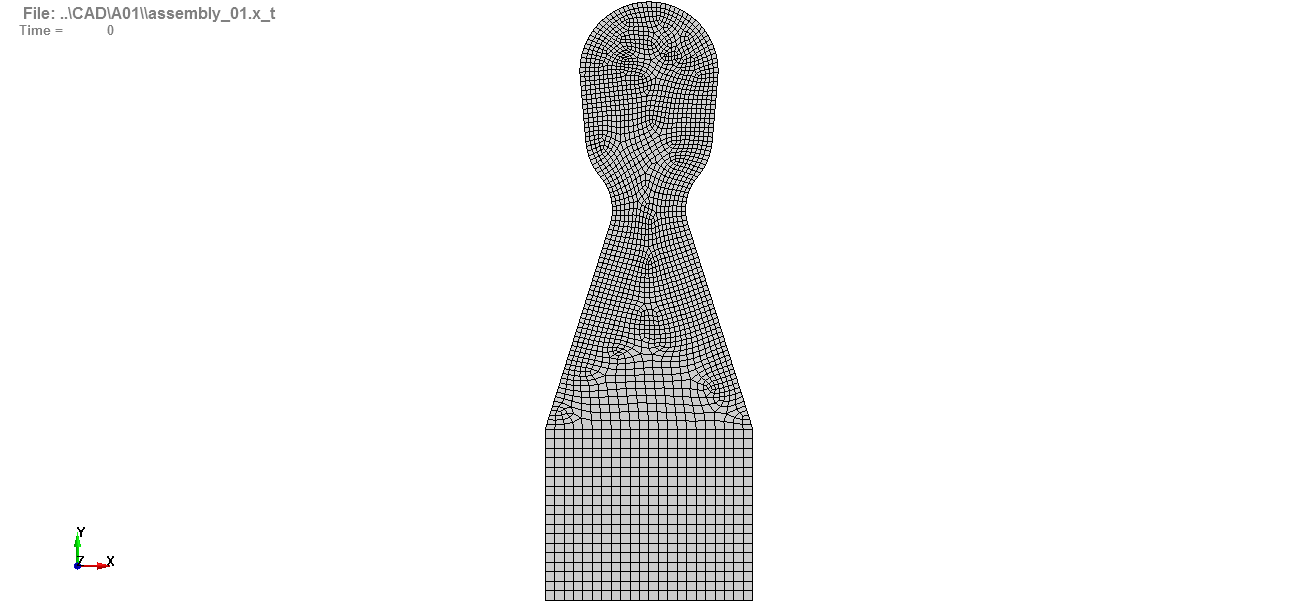
\includegraphics[width=0.60\textwidth]{src/ch3/mesh_fi_2d.png}
\captionof{figure}{Mallado del formador inferior}
\label{fig:mesh_fi_2d}
\end{center}

El resultado del mallado para los elementos formadores se puede observar en las figuras \ref{fig:mesh_fi_2d}, 
\ref{fig:mesh_fs_izq_2d}, \ref{fig:mesh_fs_der_2d}, \ref{fig:mesh_leva_izq_2d} y \ref{fig:mesh_leva_der_2d}.

\begin{figure}[H]
\centering
\begin{subfigure}[t]{0.4\textwidth}
	\centering
	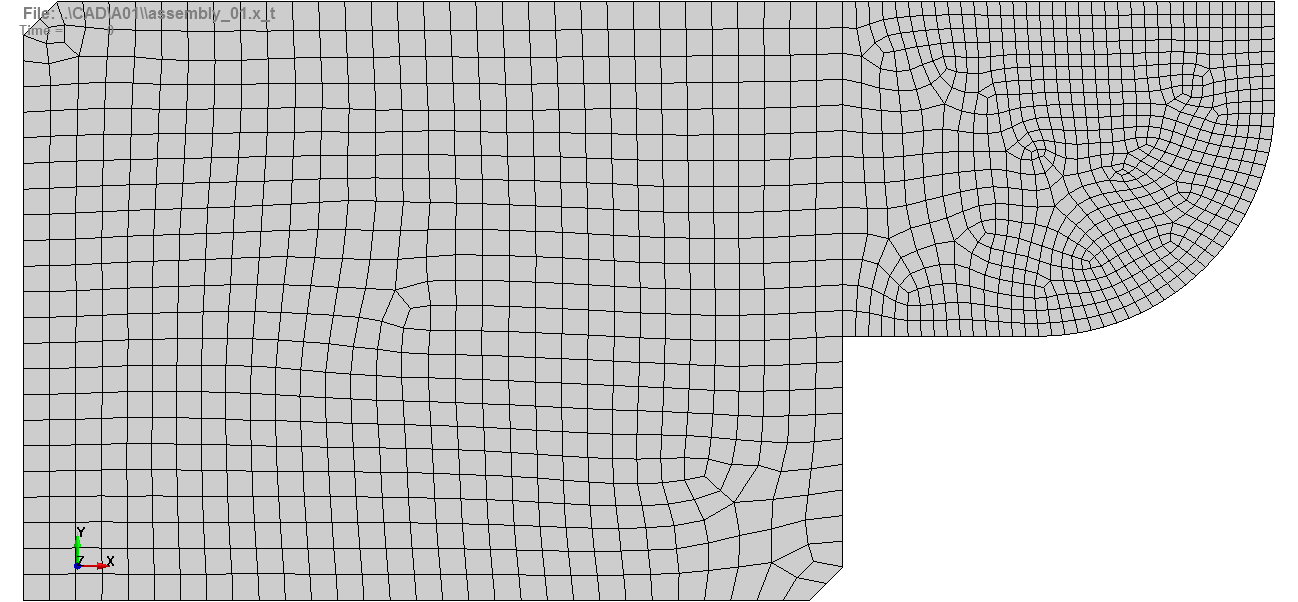
\includegraphics[width=\textwidth]{src/ch3/mesh_fs_izq_2d.png}
	\caption{}
	\label{fig:mesh_fs_izq_2d}
\end{subfigure}
~
\begin{subfigure}[t]{0.4\textwidth}
	\centering
	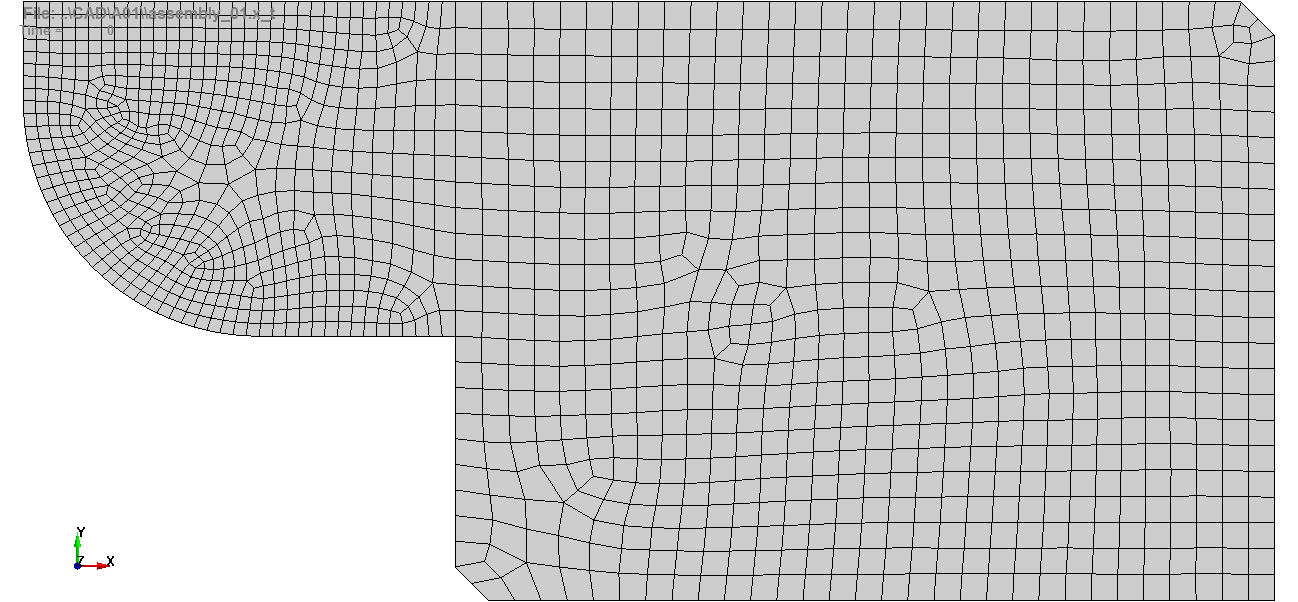
\includegraphics[width=\textwidth]{src/ch3/mesh_fs_der_2d.png}
	\caption{}
	\label{fig:mesh_fs_der_2d}
\end{subfigure}
\caption{Mallado de a) formador superior izquierdo b) formador superior derecho}
\end{figure}


\begin{figure}[H]
\centering
\begin{subfigure}[t]{0.4\textwidth}
	\centering
	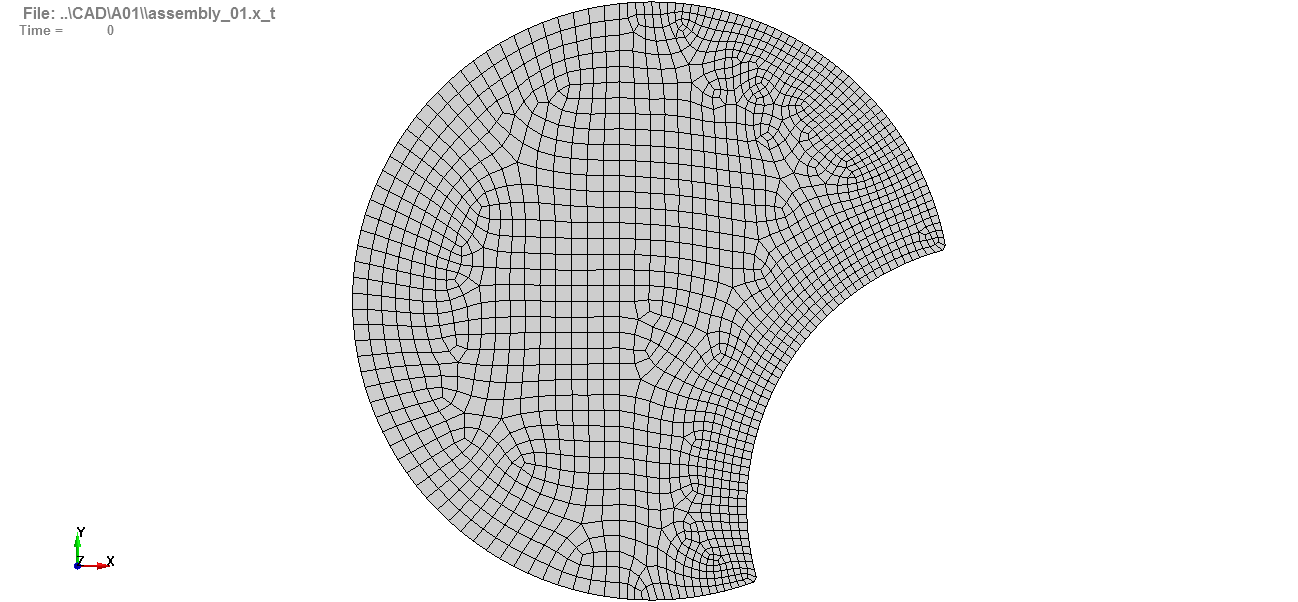
\includegraphics[width=\textwidth]{src/ch3/mesh_leva_izq_2d.png}
	\caption{}
	\label{fig:mesh_leva_izq_2d}
\end{subfigure}
~ 
\begin{subfigure}[t]{0.4\textwidth}
	\centering
	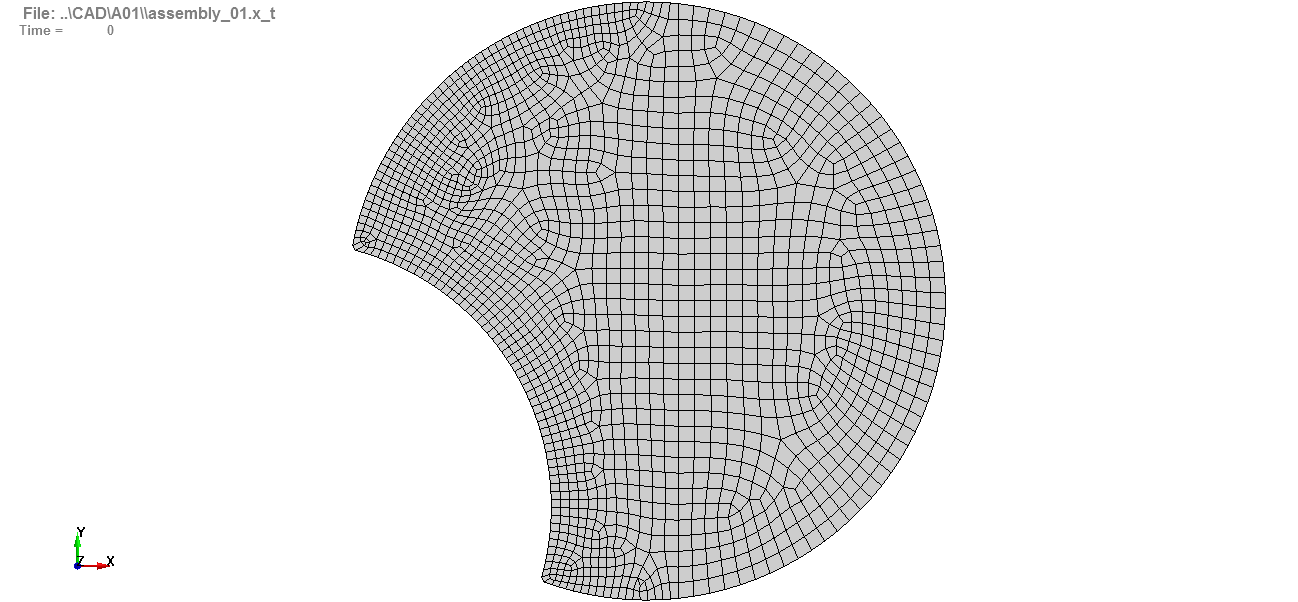
\includegraphics[width=\textwidth]{src/ch3/mesh_leva_der_2d.png}
	\caption{}
	\label{fig:mesh_leva_der_2d}
\end{subfigure}
\caption{Mallado de a) leva izquierdo b) leva derecha}
\end{figure}

Para la simulación de la segunda etapa del troquel la malla del \textit{blank} se modificó a su forma deformada 
utilizando el comando \texttt{UPGEOM} de ANSYS\faCopyright, como se describe en la sección \ref{sec:initial-stress}. 
Debido a lo anterior es evidente que el mallado del blank no se realizó de manera explícita para la segunda etapa 
y solamente se mallaron los componentes formadores del troquel. La forma deformada importada del primer paso 
se puede observar en la figura \ref{fig:mesh_deformed_blank_2d}.  \\

\begin{center}
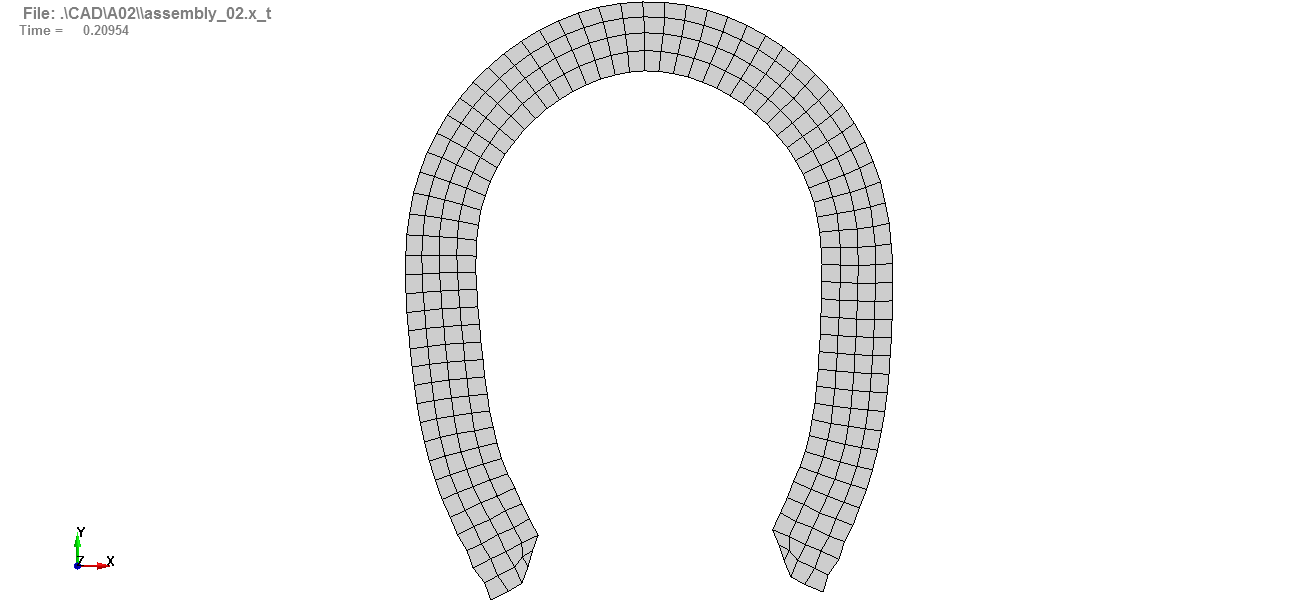
\includegraphics[width=0.5\textwidth]{src/ch3/mesh_deformed_blank_2d.png}
\captionof{figure}{Geometría deformada importada del primer paso}
\label{fig:mesh_deformed_blank_2d}
\end{center}

Como en el primer paso, los formadores de la segunda etapa del formado se mallaron con un tamaño global de 0.035 in, 
modificando el tamaño de elemento unicamente en las lineas que entran en contacto directo con el \textit{blank}.
Las figuras \ref{fig:mesh_ffi_2d}, \ref{fig:mesh_ffs_2d} y \ref{fig:mesh_perno} muestran las geometrías malladas 
para el formador final inferior, superior y el perno formador, respectivamente.

\begin{center}
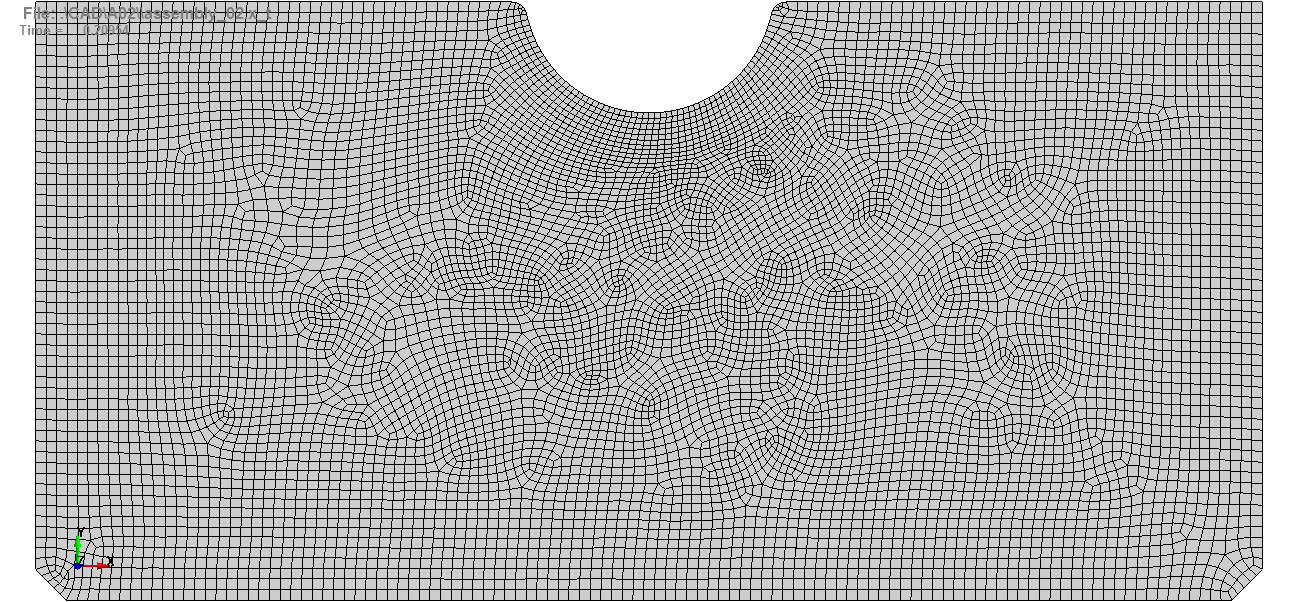
\includegraphics[width=0.5\textwidth]{src/ch3/mesh_ffi_2d.png}
\captionof{figure}{Mallado del formador final inferior}
\label{fig:mesh_ffi_2d}
\end{center}

\begin{center}
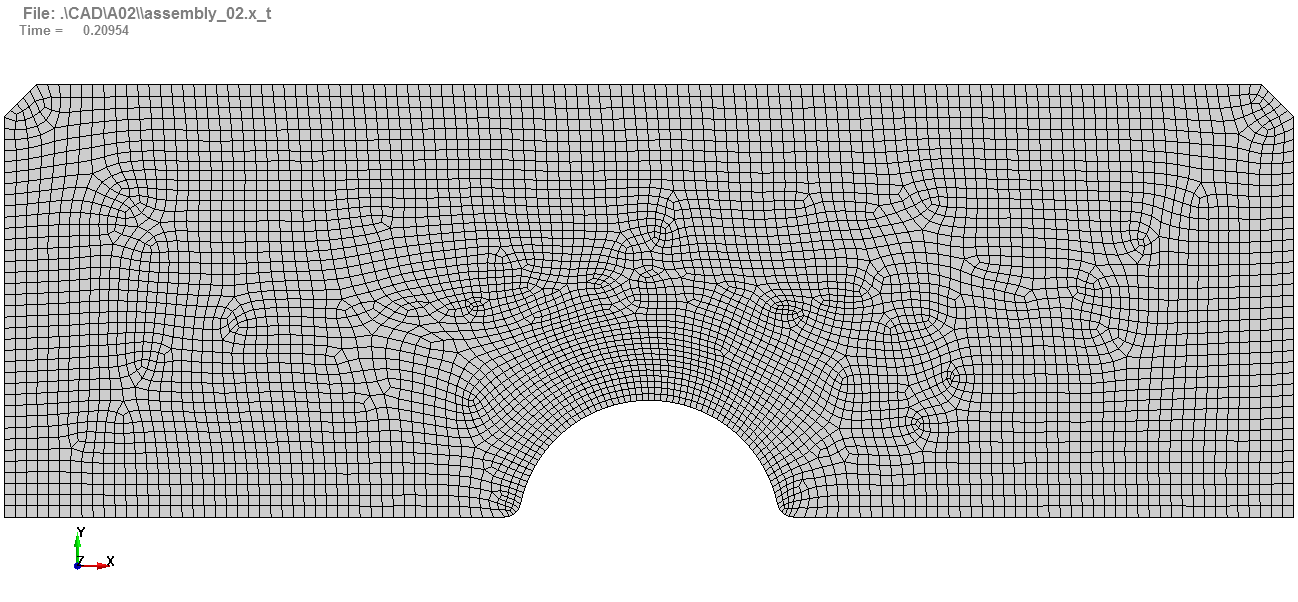
\includegraphics[width=0.5\textwidth]{src/ch3/mesh_ffs_2d.png}
\captionof{figure}{Mallado del formador final superior}
\label{fig:mesh_ffs_2d}
\end{center}

\begin{center}
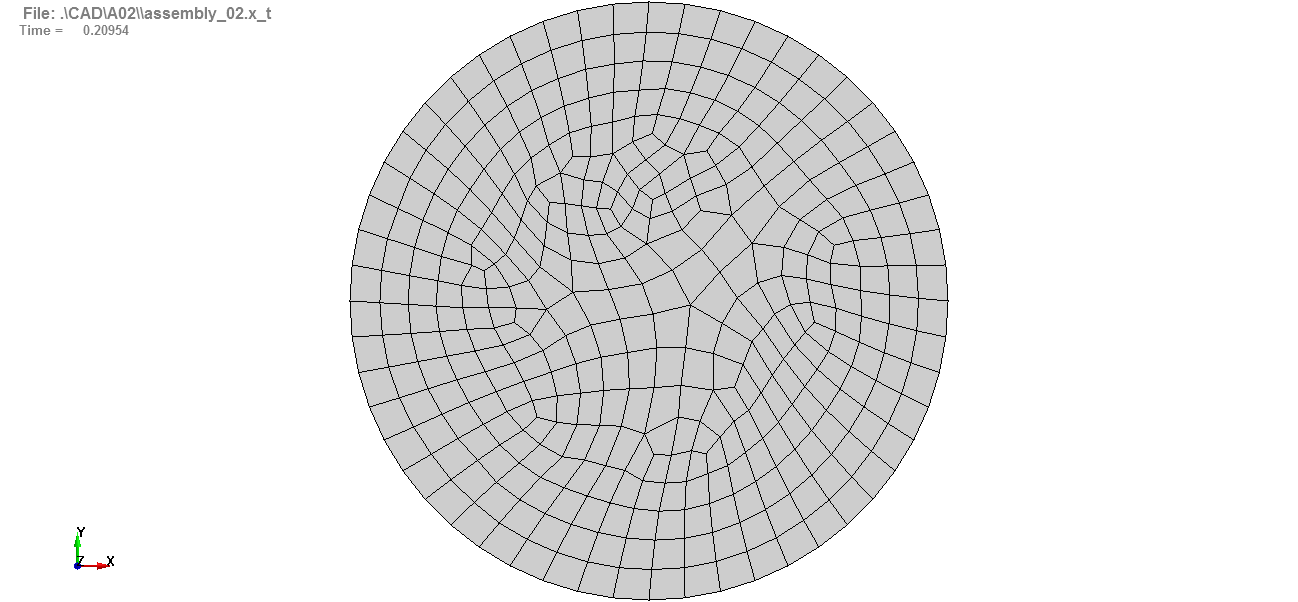
\includegraphics[width=0.35\textwidth]{src/ch3/mesh_perno_2d.png}
\captionof{figure}{Mallado del perno}
\label{fig:mesh_perno}
\end{center}


\subsubsection{Modificación de la geometría y pre-esfuerzo en la segunda etapa}\label{sec:initial-stress}

En la sección \label{sec:consideraciones-generales} se mencionó que para la segunda etapa del troquel se realizó 
una simulación de tipo \textit{restart analysis} o castellanizado literalmente: un análisis de reinicio, el cual 
básicamente es un análisis realizado como una continuación de otro, por razones que pueden ser diversas: 
análisis muy grandes que requieran subdivisiones, análisis que requieren un monitoreo o extracción de resultados 
en ciertas etapas o bien para análisis en los cuales se cambian o modifican una o más geometrías para luego 
continuarlo. Este último caso es en el cual se encuentra el proceso de formado objeto de esta tesis, dado 
que primeramente se realiza un análisis para la primera etapa y enseguida se realiza otra simulación para 
la segunda etapa del formado, misma que depende de la anterior, puesto que la geometría deformada del \textit{blank} 
es un componente de entrada.\\

El software de simulación utilizado proporciona tres tipos de \textit{restart analysis}: \textit{simple restart}, 
\textit{small restart} y \textit{full restart}. El \textit{simple restart} se utiliza cuando un análisis ha sido 
interrumpido por cuestiones ajenas al usuario y entonces se requiere continuar el análisis en el punto que 
se ha detenido. El \textit{small restart} aplica para cuando sólo se necesita hacer pequeñas modificaciones al 
análisis, tales como el tiempo de terminación, condiciones de frontera o restricciones, criterios de terminación o algunas 
especificaciones respecto a la escritura de resultados. Un análisis de tipo \textit{full restart} se utiliza 
cuando se requiere hacer cambios mayores a la base de datos del análisis, tales como modificaciones de las geometrías, 
la definición de nuevos materiales, partes, así como algunas condiciones de contacto.\\

En este caso se utilizó un análisis de tipo \textit{full restart} puesto que fue necesario borrar las geometrías 
correspondientes a los formadores del primer paso, así como la inclusión, mallado y aplicación de condiciones 
de carga y restricciones a los formadores del segundo paso, además de la definición de nuevos modelos de material 
para cada uno de los formadores del paso final.\\

Para crear un nuevo análisis de tipo \textit{full restart} se utilizó el comando \texttt{EDSTART} sobre la 
base de datos del primer análisis, utilizando un archivo de volcado o \textit{dump file} como punto de entrada, 
la sintaxis utilizada para \texttt{EDSTART} fue:

\begin{verbatim}
EDSTART,3,,,d3dump01
\end{verbatim}

Donde el número 3 indica que se hará un nuevo análisis de tipo \textit{full restart}, los siguientes dos parámetros 
se dejan vacíos para que el programa tome los valores por default, el último parámetro corresponde al nombre del 
archivo de volcado a utilizar. Normalmente los \textit{dump file} son escritos por LS-DYNA\CR al final de 
cada análisis y contienen toda la información necesaria para ejecutar un análisis de reinicio, no obstante es posible 
cambiar la periodicidad con que se escriben estos archivos mediante el comando \texttt{EDDUMP}. ~\cite{ansys-command} \\

Una vez se ejecuta el comando \texttt{EDSTART} se crea una nueva base de datos que copia toda la información de 
la anterior y entonces sobre esa nueva base de datos se puede comenzar a modificar geometrías. En este caso 
primeramente se borraron las partes correspondientes a los formadores del primer paso, se limpió la malla de 
los mismos y finalmente se borraron las geometrías correspondientes. Enseguida se importó la geometría 
correspondiente a los formadores del segundo paso, se mallaron y se definieron los nuevos modelos 
de material para cada uno de los componentes.\\

Con las geometrías de formadores malladas se procedió a modificar la geometría del \textit{blank} a su 
forma deformada, esto utilizando el comando \texttt{UPGEOM} de ANSYS\CR, cuya sintaxis es:  ~\cite{ansys-command}

\begin{verbatim}
UPGEOM, FACTOR, LSTEP, SBSTEP, FNAME, EXT
\end{verbatim}

Donde \texttt{FACTOR} es un factor de escala que en este caso fue de 1.0, dado que ambos modelos están en 
las mismas unidades de longitud, \texttt{LSTEP} y \texttt{SBSTEP} son campos que hacen referencia al número 
de paso y subpaso, respectivamente, del cual se requiere extraer la forma deformada, en este fueron valores 
de \texttt{LAST} y \texttt{LAST}, indicando que se tomará el último subpaso del último paso de carga, es decir, el instante 
final; \texttt{FNAME} y \texttt{EXT} corresponden al la ruta y extensión del archivo de resultados del cual 
se leerán los desplazamientos para realizar la modificación a las coordenadas nodales de la geometría y 
obtener la forma deformada y que normalmente corresponden al archivo de resutados (\texttt{*.rst}) del análisis previo. \\

Otra parte importante cuando se realiza un análisis de tipo \textit{full restart} es importar la distribución 
de esfuerzos en las piezas deformadas o aquellas de interés, que en este proyecto corresponde a la pieza 
de trabajo, debido a que el resto de componentes fueron modelados como rígidos y como tal no arrojan resultados 
inherentes al comportamiento mecánico. Para importar los esfuerzos desde el primer análisis y aplicarlos 
como un pre-esfuerzo en el segundo, se utilizó el comando \textit{EDIS}, colocando una instrucción como:

\begin{verbatim}
EDIS, ADD, 1, 1
\end{verbatim}

Donde el parámetro \texttt{ADD} indica que se agregarán valores, las otros dos parámetros indican el número 
de parte de donde provienen los esfuerzos y a la cual se aplicarán, de manera respectiva, en este caso 
la pieza de trabajo se identifica con el número de parte 1 en ambos análisis. \\

En la figura \ref{fig:initial_stress} se puede observar el ensamble del segundo paso, con los formadores 
mallados y la geometría deformada del \textit{blank}, además del pre-esfuerzo importado desde el resultado 
obtenido en el primer paso, cuyo máximo valor de esfuerzo de von Mises es de alrededor de 38,000 psi.

\begin{center}
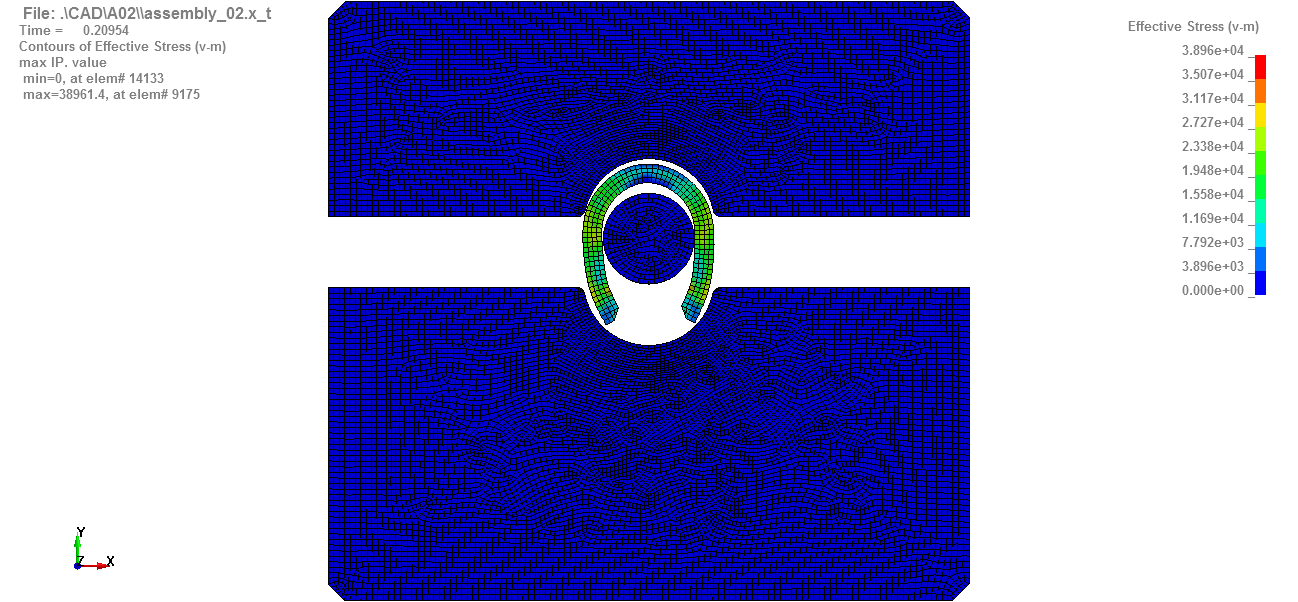
\includegraphics[width=0.85\textwidth]{src/ch3/initial_stress.png}
\captionof{figure}{Mallada deformada y esfuerzo inicial (pre-esfuerzo) aplicado}
\label{fig:initial_stress}
\end{center}

\subsubsection{Contactos}

Para el análisis bidimensional en ANSYS/LS-DYNA\CR existe un tipo de contacto especializado: 
el \textit{Automatic Single Surface 2D} (\texttt{ASS2D}) y que fue el cual se utilizó en este caso. 
Este contacto de tipo superficie única se establece cuando una superficie de un cuerpo está 
en contacto con otra o bien con él mismo, el programa determina automáticamente cuales superficies 
estarán en contacto y por tanto no es necesario definir superficies contactoras y objetivos.\\

Cuando se define el contacto de tipo \texttt{ASS2D} no es necesario especificar una a una las partes 
en contacto, sino solamente definir los coeficientes de fricción estático y dinámico. El programa de 
simulación utiliza los coeficientes de fricción estático ($FS$) y dinámico ($FD$) para la 
formulación del coeficiente friccional ($\mu_c$), que viene dado por la ecuación: ~\cite{lsdyna-manual}

\begin{equation}
\mu_c = FD + (FS - FD) e^{-DCv_{rel}}
\label{eq:frictional_coeff}
\end{equation}

Donde $DC$ es el coeficiente de decaimiento exponencial y $v_{rel}$ la velocidad relativa
entre las superficies en contacto ~\cite{lsdyna-ansys-manual}. Los valores del coeficiente de 
fricción estáticoy dinámico se establecieron en 0.2 y 0.1, respectivamente. ~\cite{carvill1993} \\

\subsubsection{Condiciones de frontera}\label{sec:condiciones-fronteras}

Para establecer las condiciones de frontera es necesario tomar en cuenta algunas  consideraciones 
básicas respecto al funcionamiento del herramental. En la primera etapa, al formar parte de un 
mismo ensamble, tanto los formadores superiores como las levas se desplazan una determinada distancia 
en dirección vertical hasta alcanzar la configuración de formado, además las levas forman 
parte de un subensamble que les permite girar en la dirección axial para lograr el predoblado, en 
cambio los formadores superiores permanecen fijos. En la segunda etapa, el formador final superior 
es el único que tiene un movimiento preescrito y el formador inferior permanece fijo en la zapata del troquel. \\

La tabla \ref{tab:bound_conds_01} resume las condiciones de carga y/o restricciones impuestas 
para la simulación del primer paso. Para el caso de los componentes del troquel, modelados como 
rígidos, las restricciones de movimiento se establecieron al momento de definir el material, 
es decir, para cada componente se definió un material específico que contiene las restricciones 
traslacionales ({\tt UX, UY, UZ}) y rotacionales ({\tt ROTX, ROTY, ROTZ}), en el \textit{script} 
incluido en el anexo \ref{sec:definicion-materiales} se muestra la definición de los materiales 
de tipo rígido para cada uno de los componentes, incluyendo las opciones de restricción como 
se indican en ~\cite{lsdyna-ansys-manual}. \\

\begin{table}[H]
\centering
\caption{Condiciones de frontera, paso 1}
\label{}
\begin{tabular}{p{4cm} p{8cm}} \hline
Geometría &  Condiciones de frontera \\
\hline
Formador inferior        & Todas las restricciones   \\
Formador superior izq.   & Desplazamiento de cuerpo rígido en Y (\texttt{RBUY}). \\
Formador superior der.   & Desplazamiento de cuerpo rígido en Y (\texttt{RBUY}). \\
Leva iquierda            & Desplazamiento de cuerpo rígido en Y (\texttt{RBUY}). Rotación en Z (\texttt{ROTZ}) libre. \\
Leva derecha             & Desplazamiento de cuerpo rígido en Y (\texttt{RBUY}). Rotación en Z (\texttt{ROTZ}) libre. \\
Blank                    & Ninguna restricción aplicada. \\
\hline
\end{tabular}
\label{tab:bound_conds_01}
\end{table}

Las condiciones de desplazamiento de cuerpo rígido para los formadores superiores y levas 
se establecieron utilizando arreglos unidimensionales tanto para el historial de tiempo 
como para el de desplazamientos. Se optó por utilizar una curva de carga de tipo 
\textit{smooth-step} ~\cite{smooth-step-wiki} tal como se recomienda para análisis 
de tipo dinámico-explícito en simulaciones de estampado ~\cite{input-param-lsdyna}, 
este tipo de curva se caracteriza por tener un crecimiento lento al principio y 
final de su intervalo,  implicando una velocidad \textit{reducida} de los formadores al principio y final 
del recorrido, con la finalidad de que esto facilite la estabilización y convergencia
del análisis. \\

La función de tipo \textit{smooth-step} utilizada tiene la forma general $f(t) = A(Bt^2 - Ct^3)$, 
donde $A$, $B$ y $C$ son constantes a ajustar para el requerimiento de desplazamiento total y el 
tamaño del intervalo. En la tabla \ref{tab:smooth_step_constants} se muestran los valores para 
las constantes utilizados en cada uno de los pasos de la simulación. Además, para cada 
una de las dos etapas de simulación se necesitó definir dos funciones, una para el proceso 
de carga y otra para la descarga, quedando de manera general una función definida a trozos como sigue:

\begin{equation}
f(t) = \left\{\begin{matrix}
A(Bt^2 - Ct^3) \,\,\,\,\,\, &  \text{para} \,\, t \leq 0.1 \\
-A(Bt^2 - Ct^3) + K \,\,\,\,\,\,& \text{para} \,\, t > 0.1 \\
\end{matrix}\right.
\end{equation}

Donde K es el valor mínimo que toma la función, es decir, $K = f(t=0.1)$. Las gráficas de 
las curvas resultantes para ambos pasos de la simulación se muestran en las figuras 
\ref{fig:smooth_displacement_01} y \ref{fig:smooth_displacement_02}.

\begin{table}[H]
\centering
\caption{Valores para las constantes A, B y C}
\label{}
\begin{tabular}{p{3cm} p{2cm} p{2cm}} \hline
Parámetro & 1er. paso & 2do. paso \\
\hline
A & -1.22 & -0.225 \\
B & $1.15\text{x}10^{-4}$ & $1.15\text{x}10^{-4}$ \\
C & $3.8\text{x}10^{-7}$ & $3.8\text{x}10^{-7}$ \\
\hline
\end{tabular}
\label{tab:smooth_step_constants}
\end{table}

\begin{figure}[H]
\centering
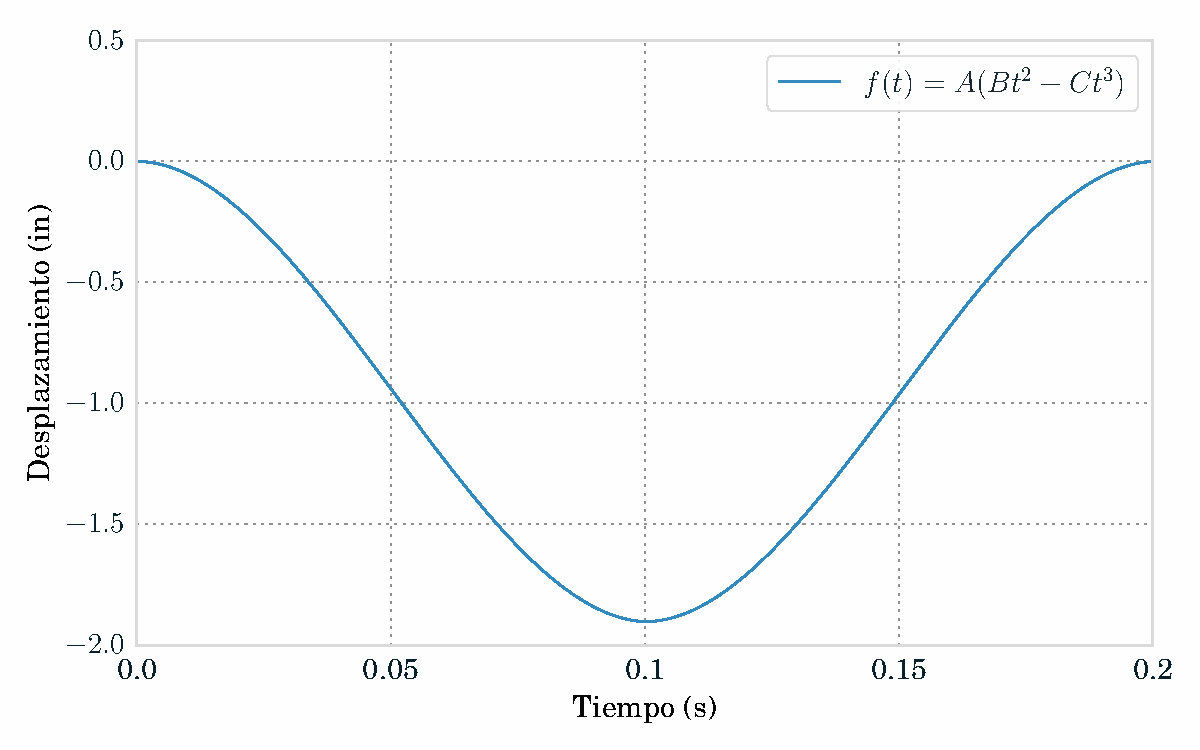
\includegraphics[width=0.75\textwidth]{src/ch3/smooth_displacement_01.pdf}
\captionof{figure}{Vector de tiempo desplazamiento, paso 1}
\label{fig:smooth_displacement_01}
\end{figure}

En la tabla \ref{tab:bound_conds_02} se resumen las condiciones de carga y restricciones aplicadas 
al ensamble del segundo paso. La imposición de esas condiciones se hicieron de igual manera que para 
lo descrito en el primer ensamble, variando evidentemente la relación tiempo-desplazamiento de los 
formadores, misma que ya se ha descrito.

\begin{table}[H]
\centering
\caption{Condiciones de frontera, paso 2}
\label{}
\begin{tabular}{p{4cm} p{8cm}} \hline
Geometría &  Condiciones de frontera \\
\hline
Formador inferior        & Todas las restricciones   \\
Formador superior        & Desplazamiento de cuerpo rígido en Y (\texttt{RBUY}). \\
Perno formador           & Desplazamiento en Y (\texttt{UY}) libre  \\
Blank                    & Ninguna restricción aplicada. \\
\hline
\end{tabular}
\label{tab:bound_conds_02}
\end{table}

\begin{figure}[H]
\centering
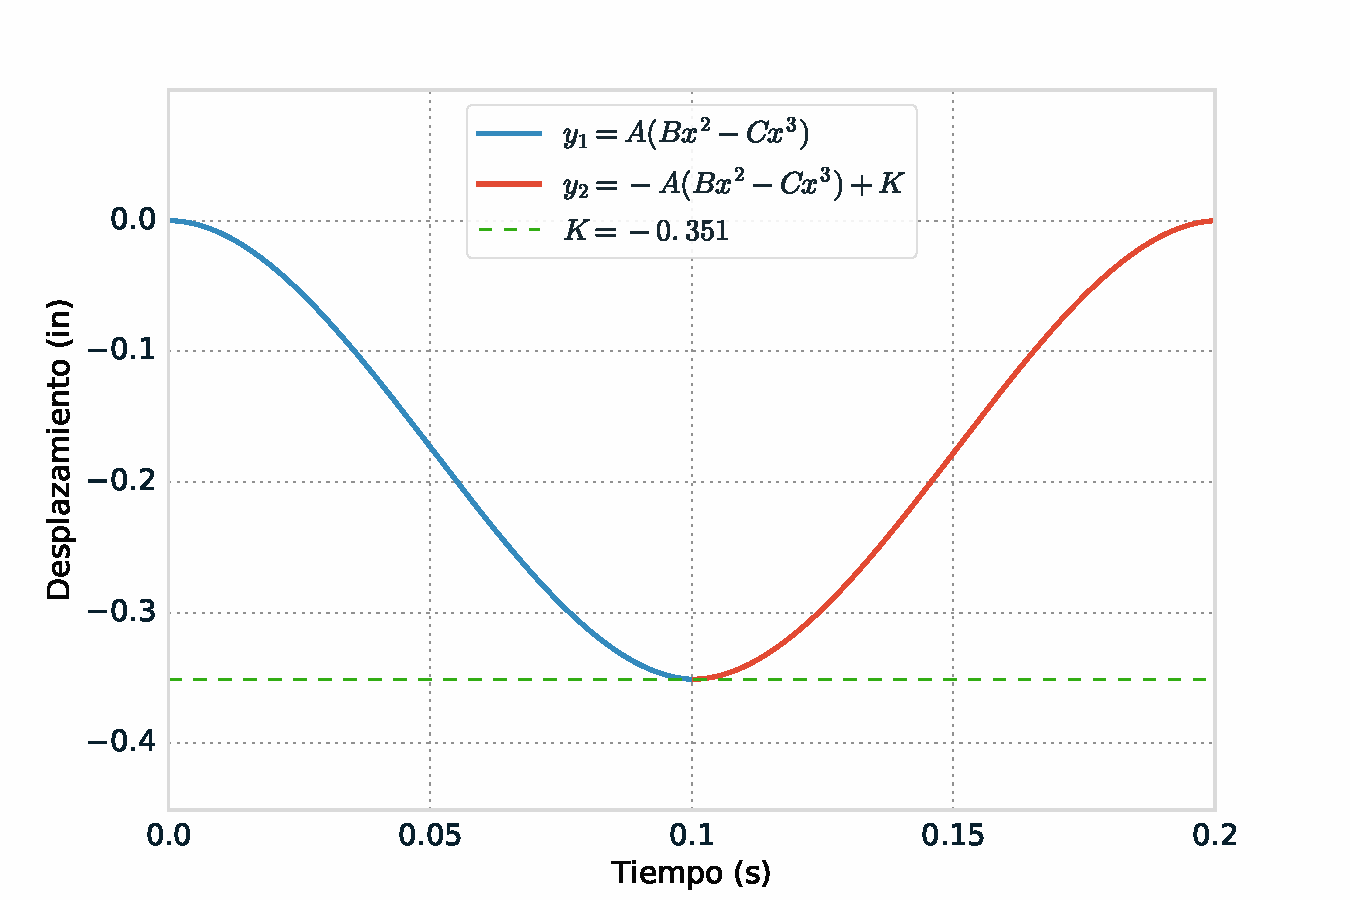
\includegraphics[width=0.75\textwidth]{src/ch3/smooth_displacement_02.pdf}
\captionof{figure}{Vector de tiempo desplazamiento, paso 2}
\label{fig:smooth_displacement_02}
\end{figure}


% \subsubsection{Escalamiento de masa}\label{sec:mass-scaling}


\subsection{Análisis tridimensional}

\subsubsection{Mallado}

Para el mallado de la pieza de trabajo se utilizó el elemento \texttt{SOLID164} 
( ver figura \ref{fig:solid164} ), el cual es un sólido de 8 nodos, que puede ser utilizado con el modelo 
constitutivo descrito en la sección anterior. Este elemento utiliza, por defecto, integración reducida 
(un punto de integración), el cual tiene la ventaja de reducir el tiempo de cómputo y adiciona 
robustez para el caso de grandes deformaciones ~\cite{lsdyna-ansys-manual}, no obstante puede presentar 
la desventaja de propiciar la inclusión de los modos de Hourglass en la solución, implicando que 
se obtenga una malla deformada con apariencia corrugada.

\begin{center}
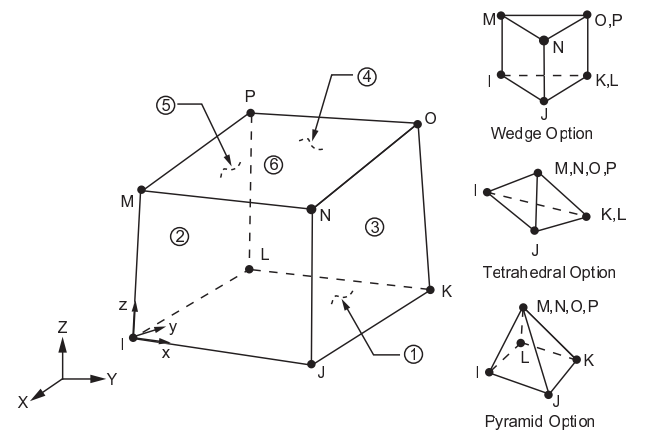
\includegraphics[scale=0.65]{src/ch3/solid164.png}
\captionof{figure}{Elemento \texttt{SOLID164}}
\label{fig:solid164}
\end{center}

En los componentes del troquel se mallaron solamente las áreas que están en contacto directo con el 
\textit{blank} durante el proceso de formado, con la finalidad de reducir el número de elementos del modelo. 
Se utilizaron elementos \texttt{SHELL163} para realizar el mallado. Los parámetros requeridos para 
este elemento se indican en la tabla \ref{tab:shell_param}.

\begin{center}
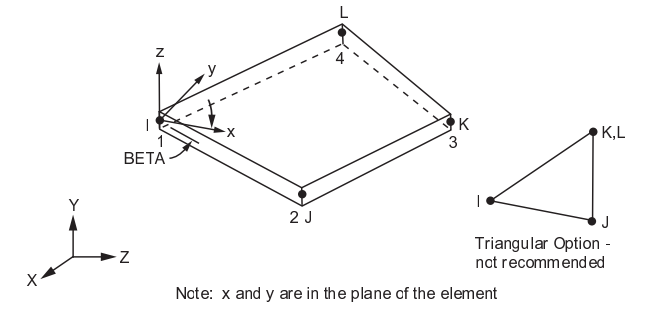
\includegraphics[scale=0.65]{src/ch3/shell163.png}
\captionof{figure}{Elemento SHELL163}
\label{fig:shell163}
\end{center}


% Tabla de propiedades para elemento SHELL163
\begin{table}[h]
\centering
\caption{Parámetros utilizados para el elemento SHELL163}
\label{}
\begin{tabular}{p{6cm} p{6cm}} \hline
Parámetros & Valores \\
\hline
General shell formulation & Belytschko-Tsay \\
Membrane element formulation & Belytschko-Tsay Membrane \\
Triangular shell formulation & $C^0$ triangular shell \\
\hline
\end{tabular}
\label{tab:shell_param}
\end{table}


% Tabla de constantes reales para elemento SHELL163
\begin{table}[h]
\centering
\caption{Constantes reales para el elemento SHELL163}
\label{}
\begin{tabular}{p{6cm} p{3cm}} \hline
Parámetros & Valores \\
\hline
Factor cortante (SHRF) & 5/6 \\
Puntos de integración (NIP) & 1 \\
Espesor en nodo 1 (T1) & 0.2 \\
Espesor en nodo 2 (T2) & 0.2 \\
Espesor en nodo 3 (T3) & 0.2 \\
Espesor en nodo 4 (T4) & 0.2 \\
\hline
\end{tabular}
\label{tab:shell_param}
\end{table}


En el \textit{blank} se utilizó un tamaño global de elemento de 0.03 in, y 0.035 in en el caso de las partes 
rígidas, exceptuando las áreas que están directamente en contacto con el \textit{blank}, en cuyo caso se hizo 
un refinamiento, dejando el tamaño global en 0.02 in. En el \textit{blank} fue necesario segmentar en cuatro 
volúmenes, para permitir un mallado más uniforme (ver figura \ref{fig:blank_seg} ).


% Partición del blank
\begin{center}
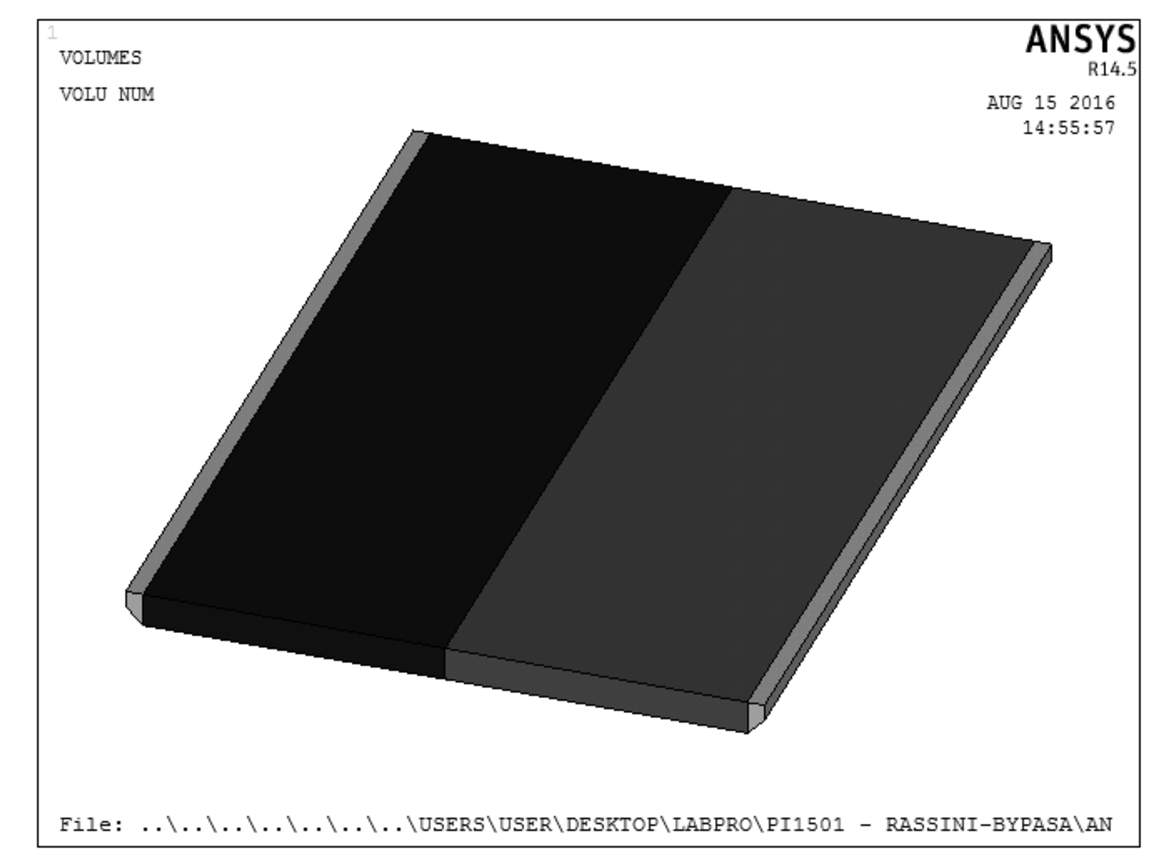
\includegraphics[width=0.5\textwidth]{src/ch3/blank_segmentado.pdf}
\captionof{figure}{Blank segmentado en cuatro regiones}
\label{fig:blank_seg}
\end{center}


% Mallado del blank


\begin{figure}[H]
\centering
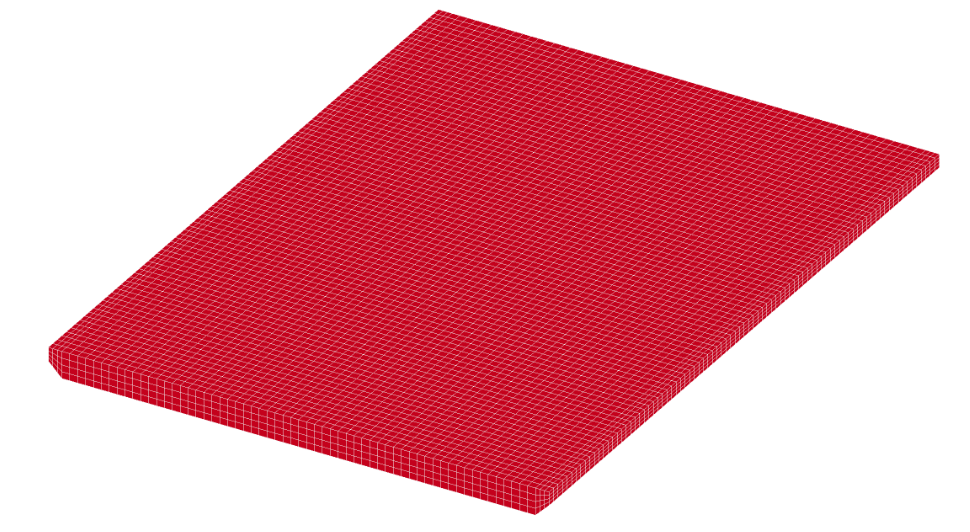
\includegraphics[width=0.5\textwidth]{src/ch3/mesh_blank.png}
\label{fig:mesh_blank}
\caption{Mallado del blank}
\end{figure}


\begin{figure}[H]
\centering
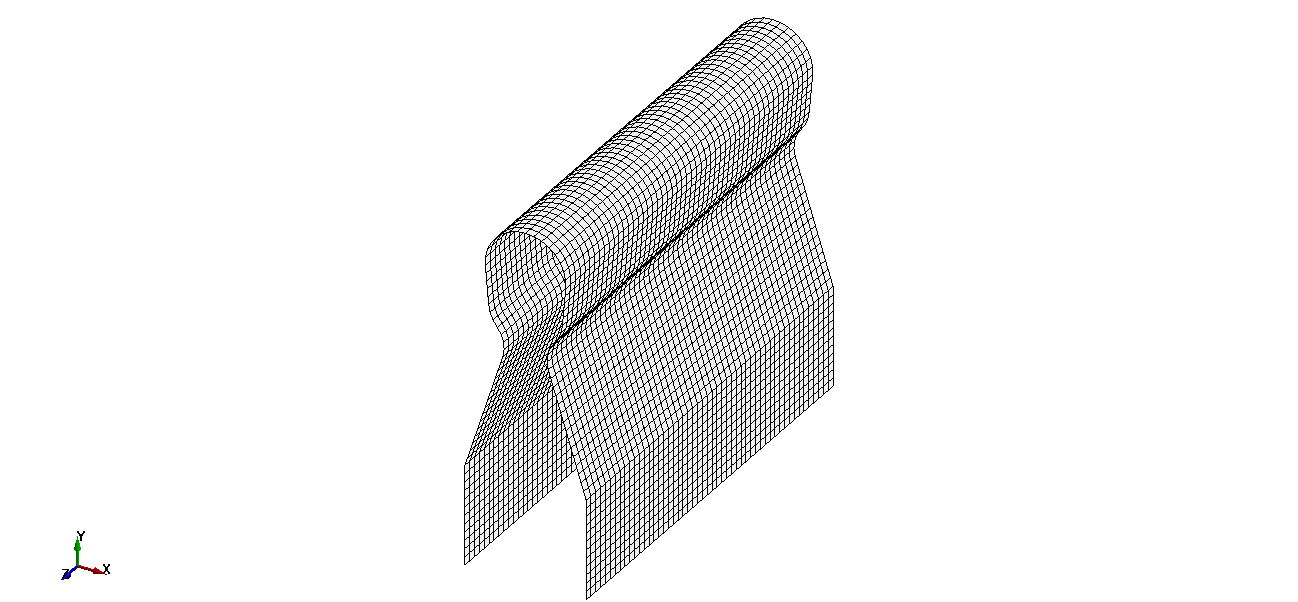
\includegraphics[width=0.5\textwidth]{src/ch3/mesh_fi.png}
\caption{Mallado del formador inferior}
\label{fig:mesh_fi}
\end{figure}

\begin{figure}[H]
\centering
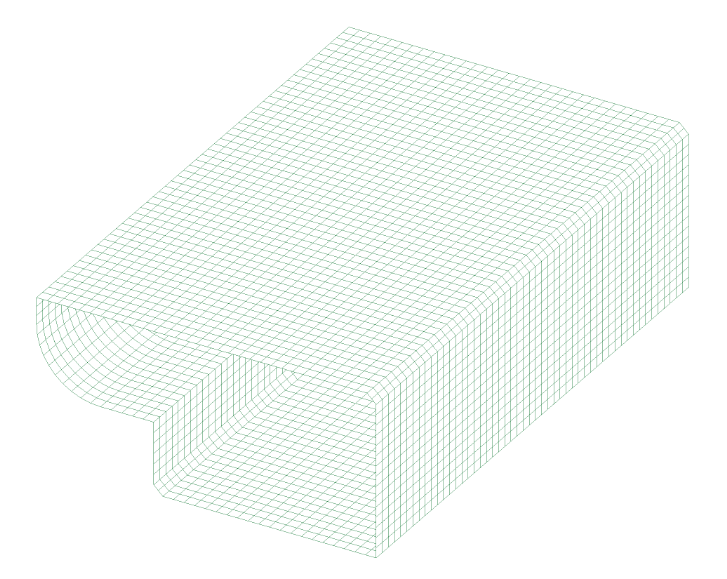
\includegraphics[width=0.5\textwidth]{src/ch3/mesh_fs.png}
\caption{Mallado del formador superior}
\label{fig:mesh_fi}
\end{figure}

\begin{figure}[H]
\centering
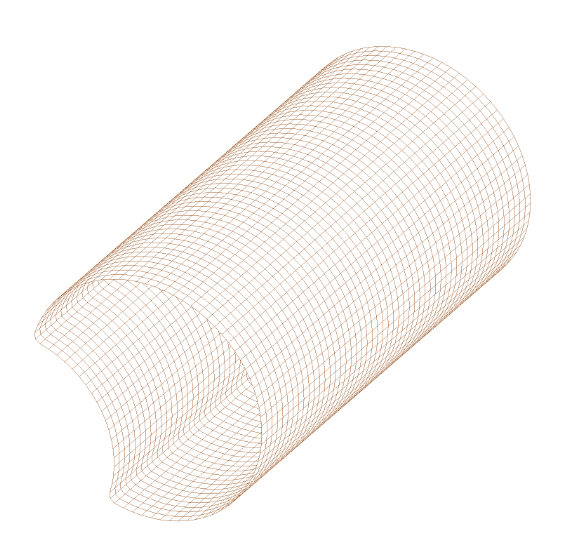
\includegraphics[width=0.5\textwidth]{src/ch3/mesh_leva.png}
\caption{Mallado de la leva}
\label{fig:mesh_fi}
\end{figure}


% \begin{figure}[!h]
% \centering
% \begin{subfigure}[t]{0.3\textwidth}
% \centering
% 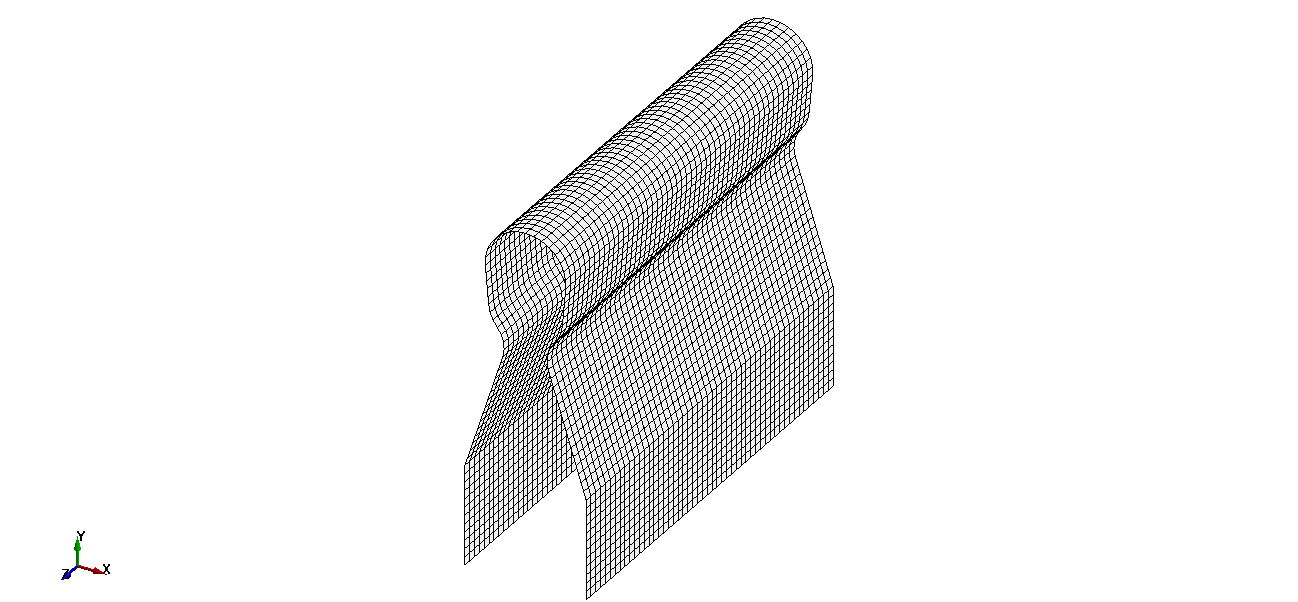
\includegraphics[width=\textwidth]{src/ch3/mesh_fi.png}
% \caption{}
% \label{fig:mesh_fi}
% \end{subfigure}
% ~ 
% \begin{subfigure}[t]{0.3\textwidth}
% \centering
% 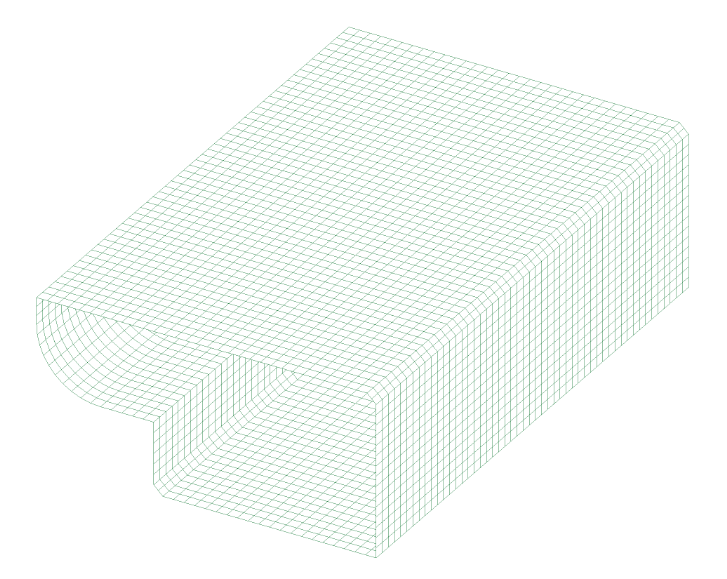
\includegraphics[width=\textwidth]{src/ch3/mesh_fs.png}
% \caption{}
% \label{fig:mesh_fs}
% \end{subfigure}
% ~ 
% \begin{subfigure}[t]{0.3\textwidth}
% \centering
% 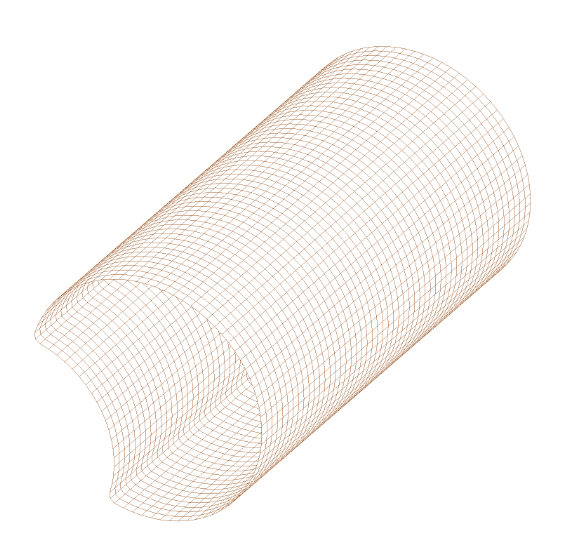
\includegraphics[width=\textwidth]{src/ch3/mesh_leva.png}
% \caption{}
% \label{fig:mesh_leva}
% \end{subfigure}

% \caption{Mallado de a) formador inferior b) formador superior c) leva}
% \end{figure}


% %  Partes 
% \begin{figure}[!h]
% \centering
% 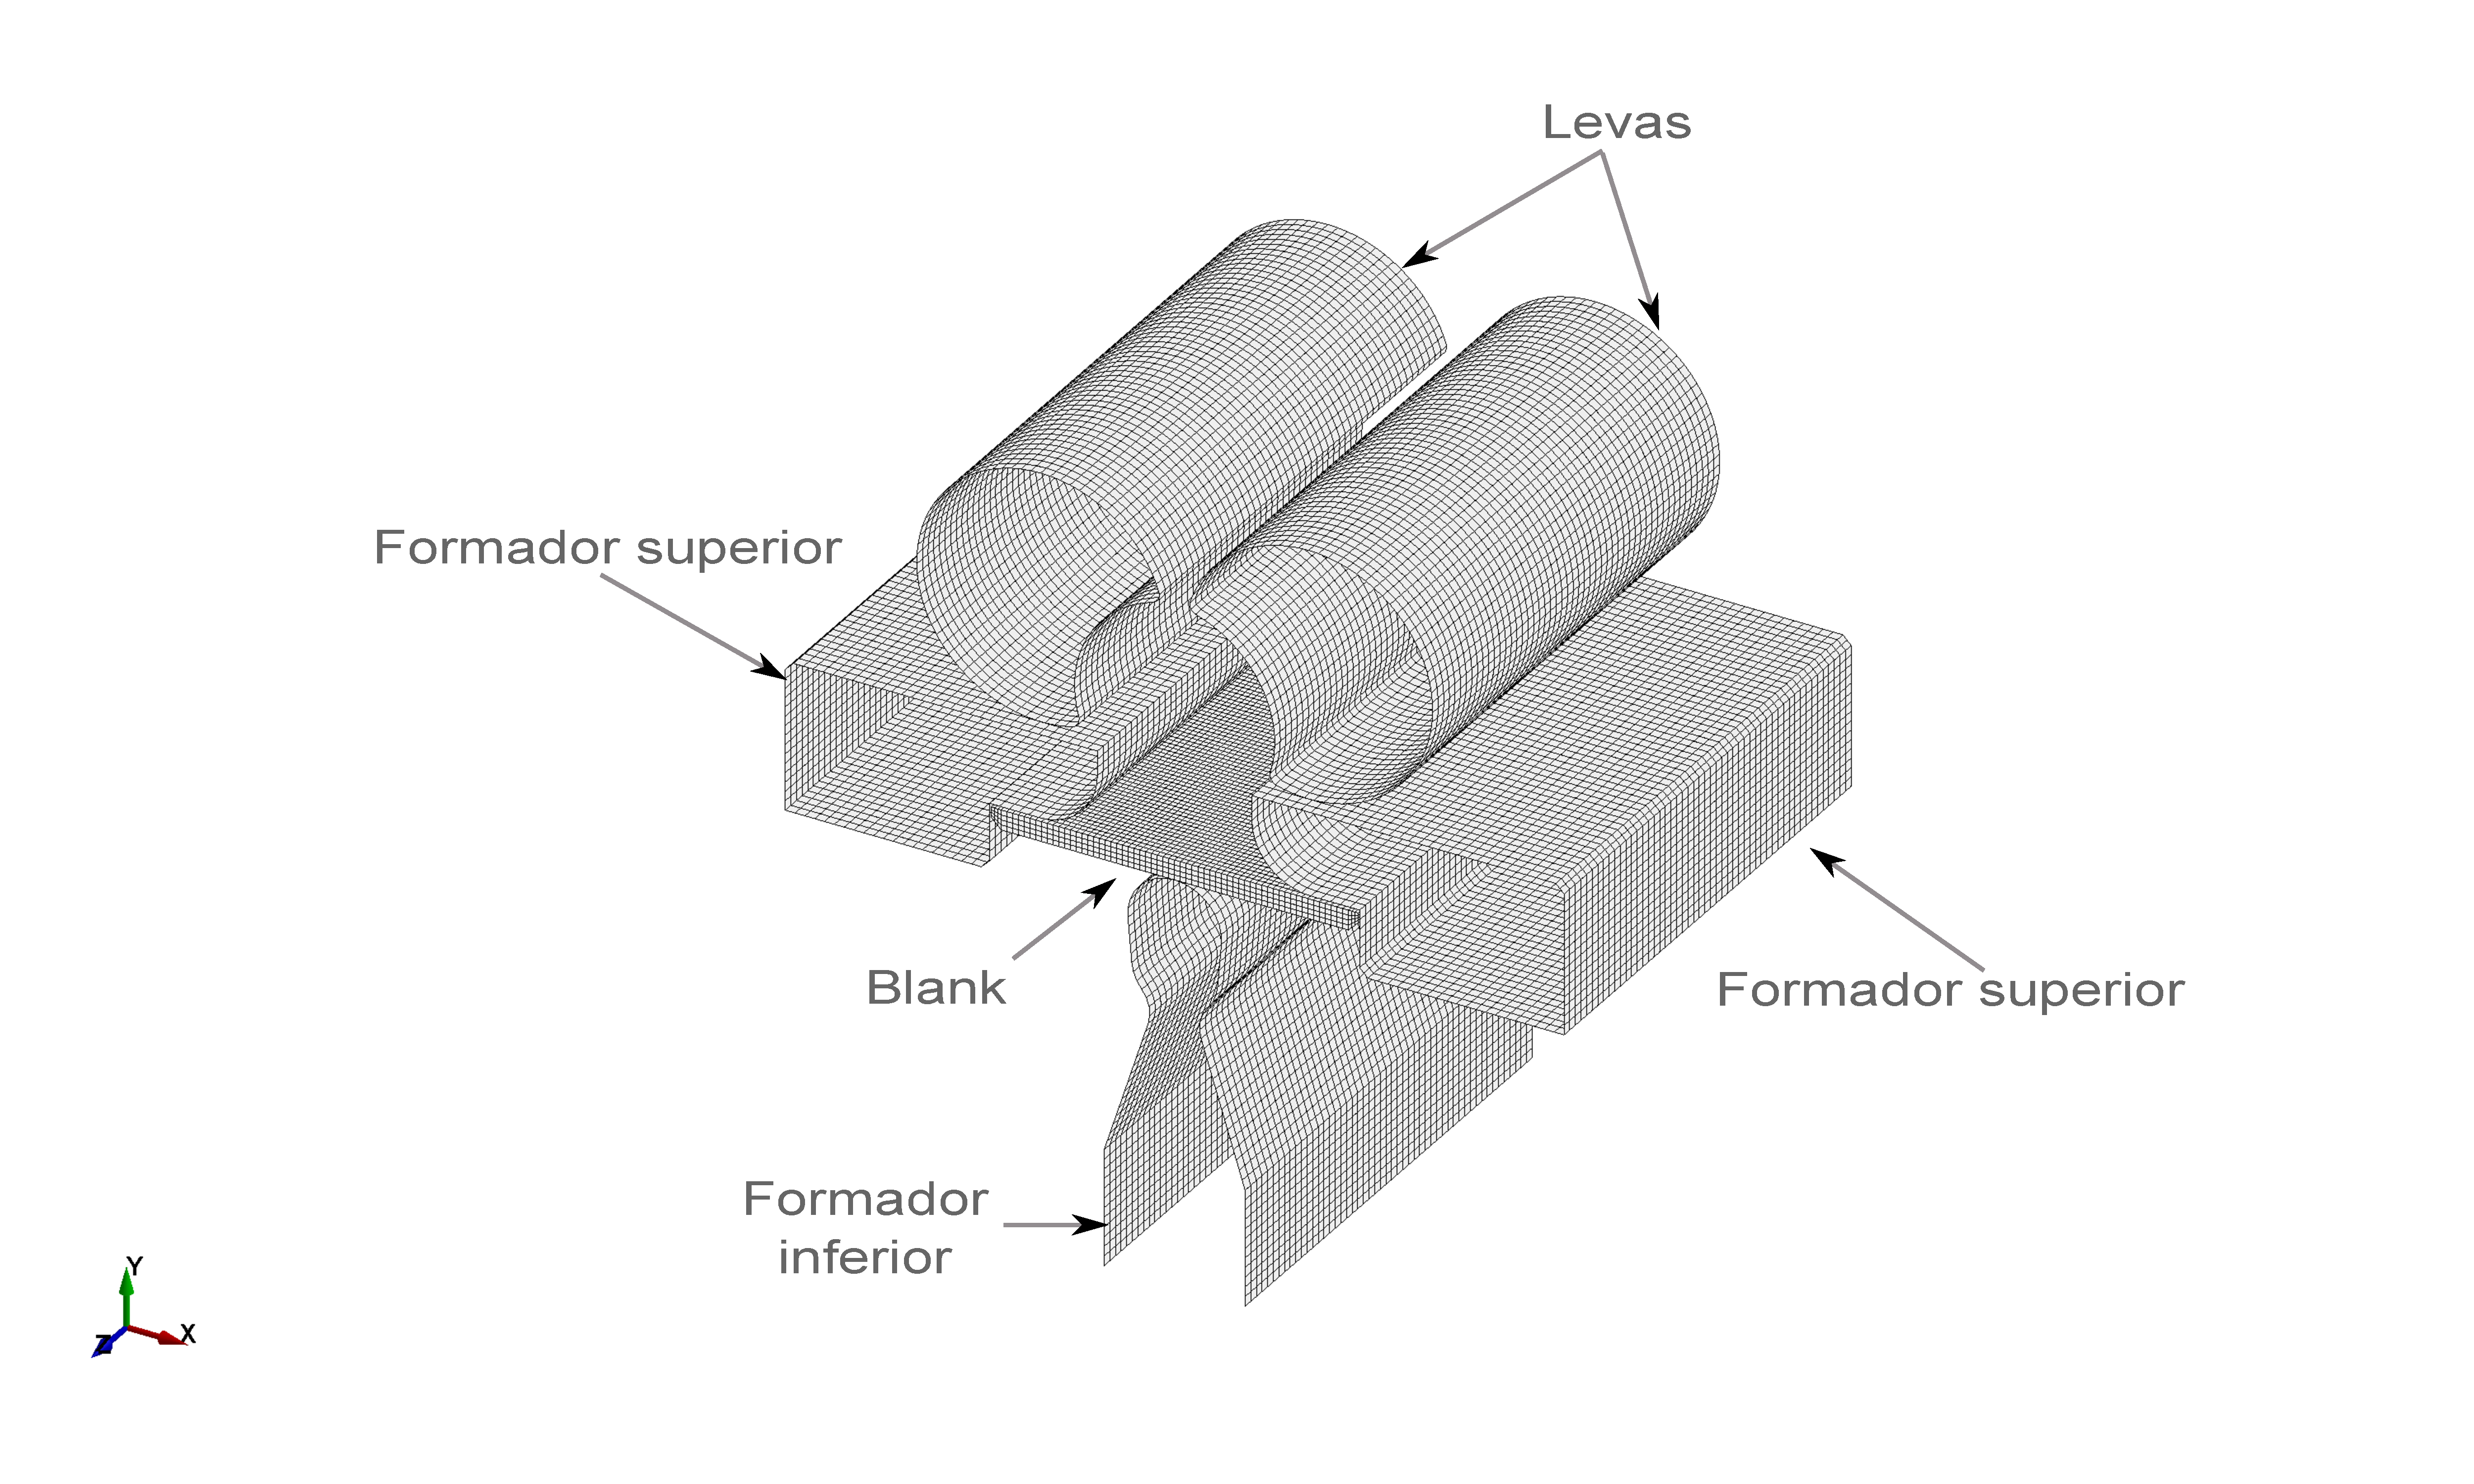
\includegraphics[width=0.8\textwidth]{src/ch3/parts_01.pdf}
% \caption{Partes del ensamble 1}
% \label{fig:parts_01}
% \end{figure}

% En las tabla \ref{tab:elements_and_nodes} se muestra el número de nodos y elementos obtenidos 
% para cada uno de los ensambles.

% \begin{table}[h]
% \centering
% \caption{Número de nodos y elementos}
% \label{}
% \begin{tabular}{p{2cm} p{2cm} p{2cm}} \hline
%  & Nodos & Elementos \\
% \hline
% Paso 1 & 52285 & 45348 \\
% Paso 2 & 48884 & 42264 \\
% \hline
% \end{tabular}
% \label{tab:elements_and_nodes}
% \end{table}

Al igual que en el primer ensamble, los formadores y/o componentes del herramental, se 
mallaron por áreas utilizando elementos \texttt{SHELL163}. En el caso de la pieza de trabajo, 
esta se importó en su configuración deformada del análisis del primer paso, incluyendo 
además la distribución de esfuerzos. En la figura \ref{fig:mesh_blank_02} se observa 
la malla deformada del blank. El mallado de cada uno de los componentes del troquel 
se puede observar en las figuras \ref{fig:mesh_ffi}, \ref{fig:mesh_ffs} y \ref{fig:mesh_perno}.

% \begin{figure}[H]
% \centering
% 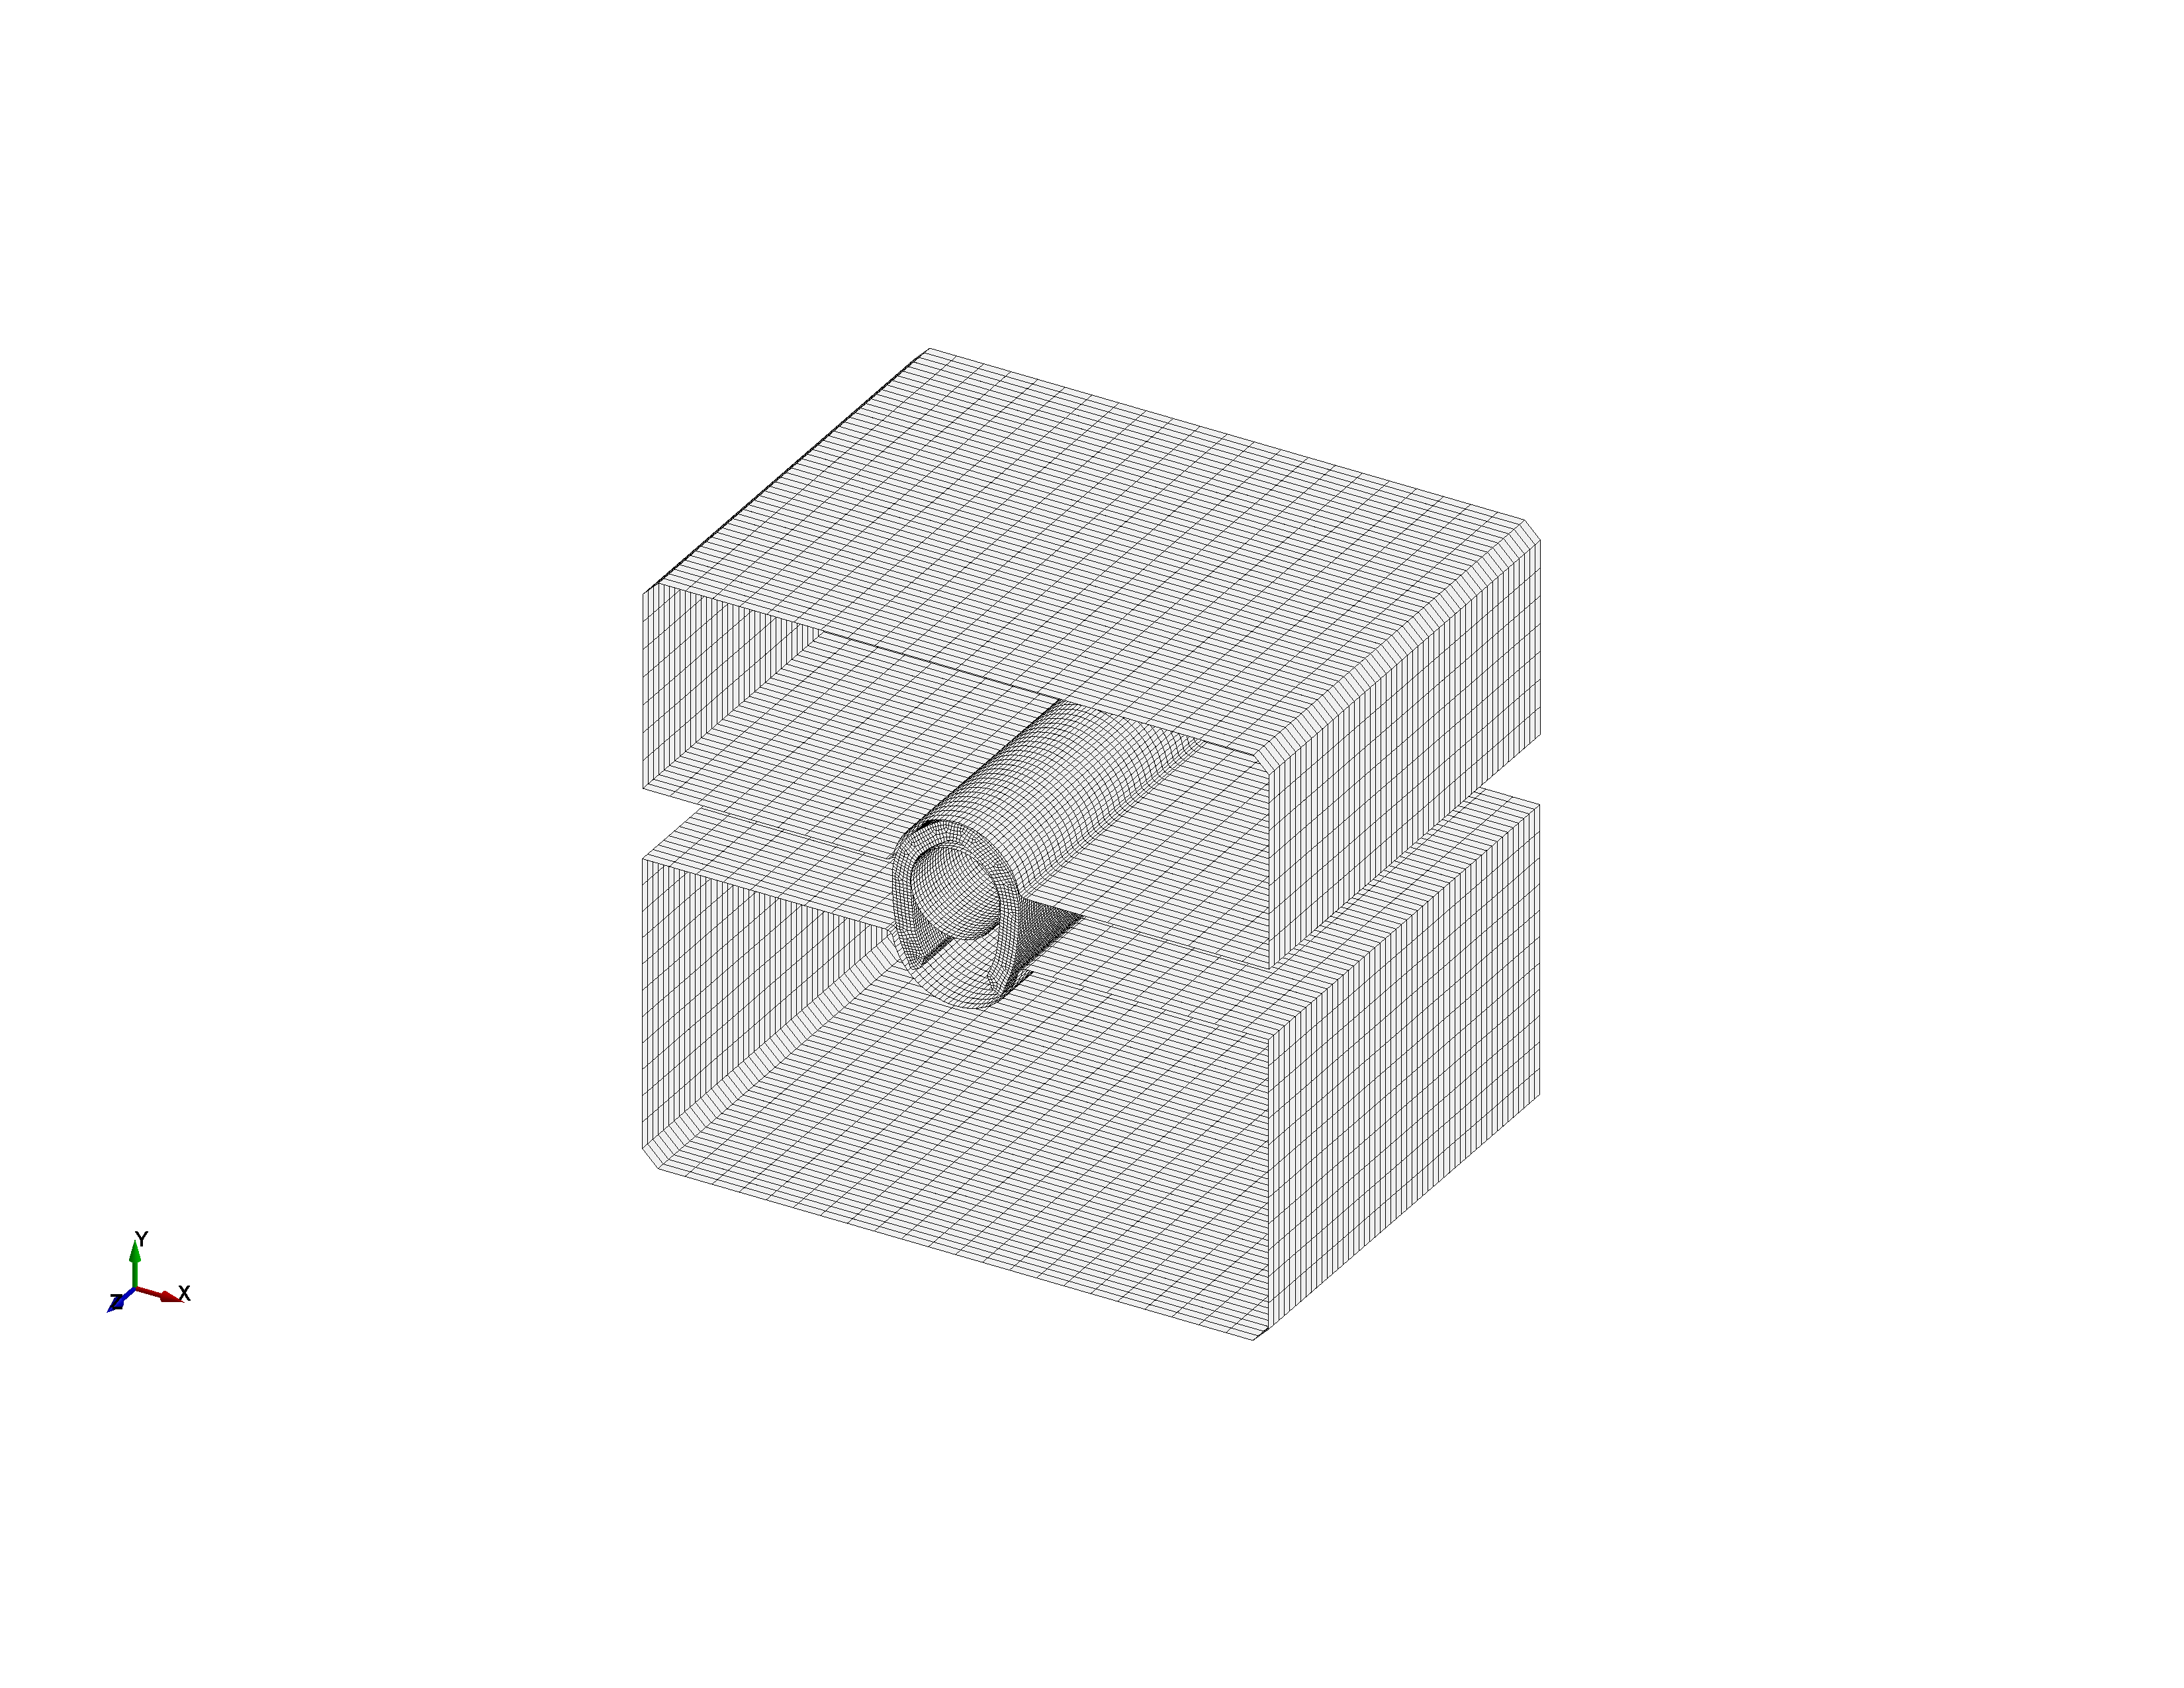
\includegraphics[width=0.6\textwidth]{src/ch3/parts_02.png}
% \caption{Mallado del segundo ensamble}
% \label{fig:parts_02}
% \end{figure}

\begin{figure}[H]
\centering
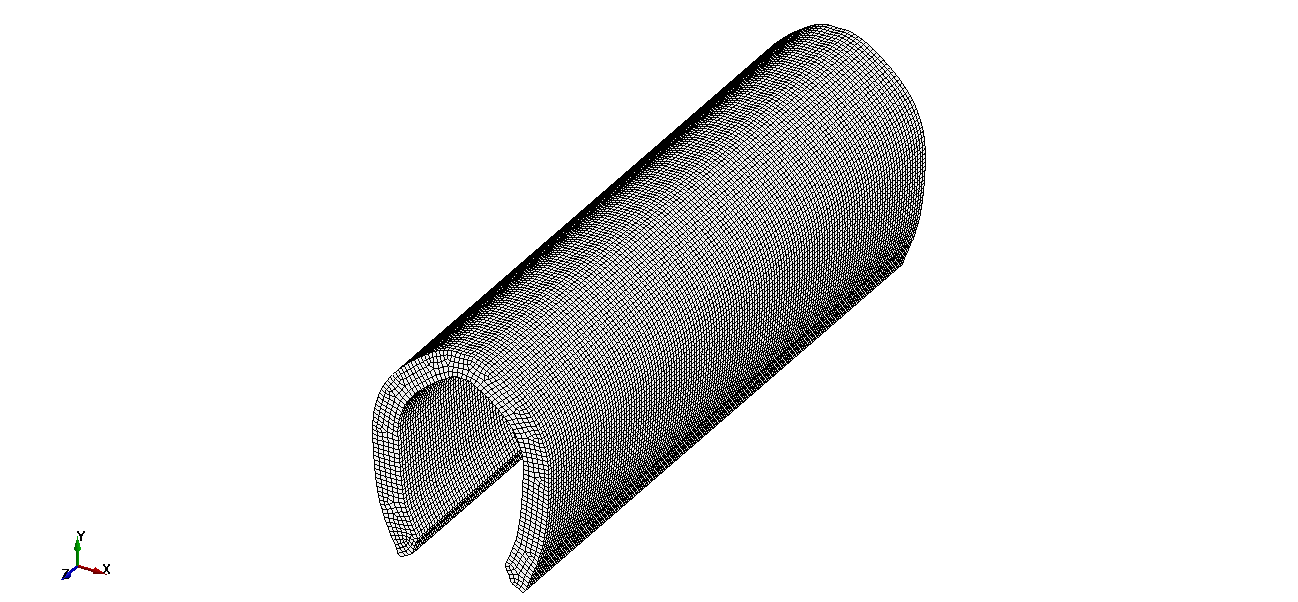
\includegraphics[width=0.5\textwidth]{src/ch3/mesh_blank_02.png}
\caption{Geometría deformada del blank importada del primer paso}
\label{fig:mesh_blank_02}
\end{figure}

\begin{figure}[H]
\centering
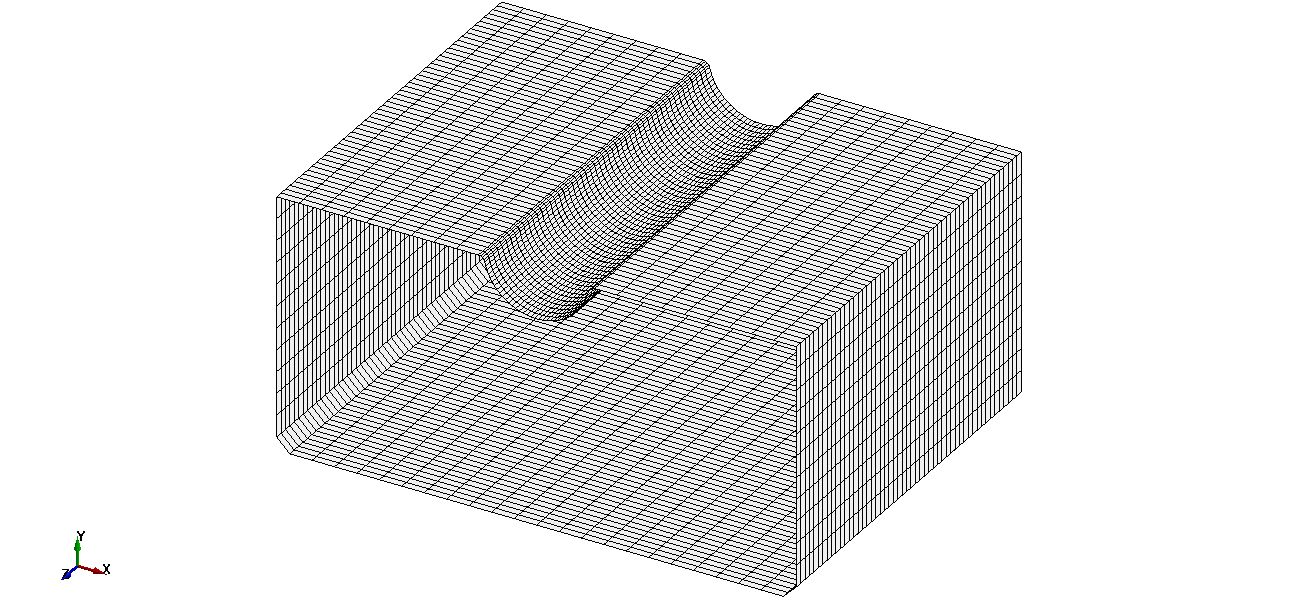
\includegraphics[width=0.5\textwidth]{src/ch3/mesh_ffi.png}
\caption{Mallado del formador final inferior}
\label{fig:mesh_ffi}
\end{figure}

\begin{figure}[H]
\centering
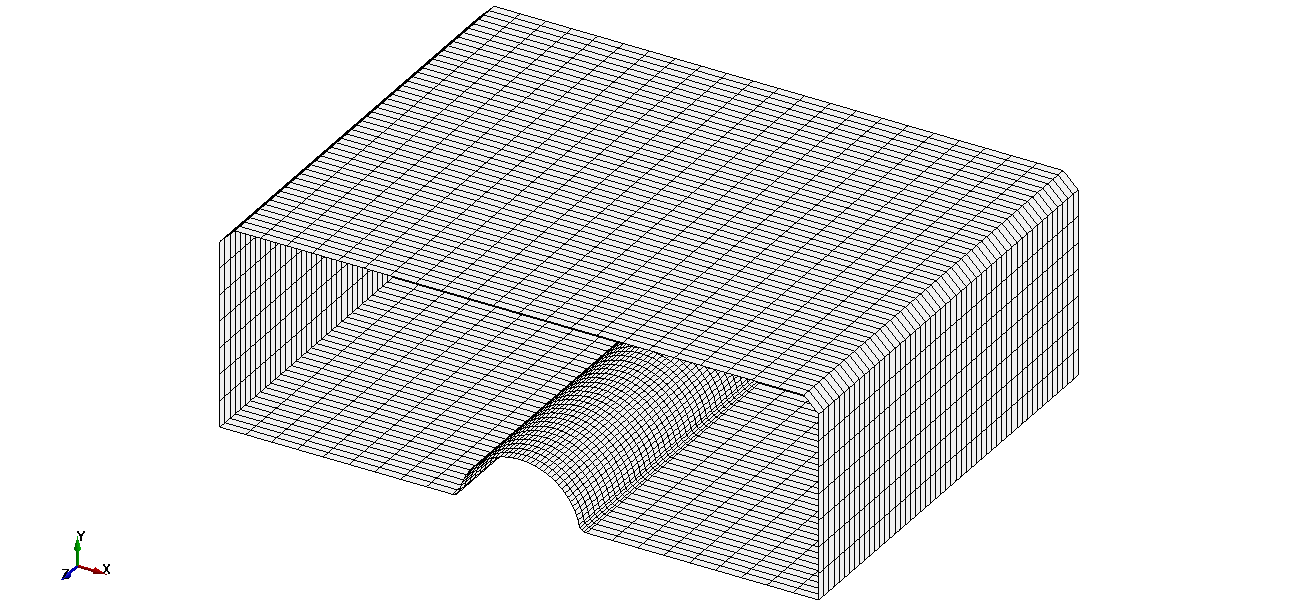
\includegraphics[width=0.5\textwidth]{src/ch3/mesh_ffs.png}
\caption{Mallado del formador final superior}
\label{fig:mesh_ffs}
\end{figure}

\begin{figure}[H]
\centering
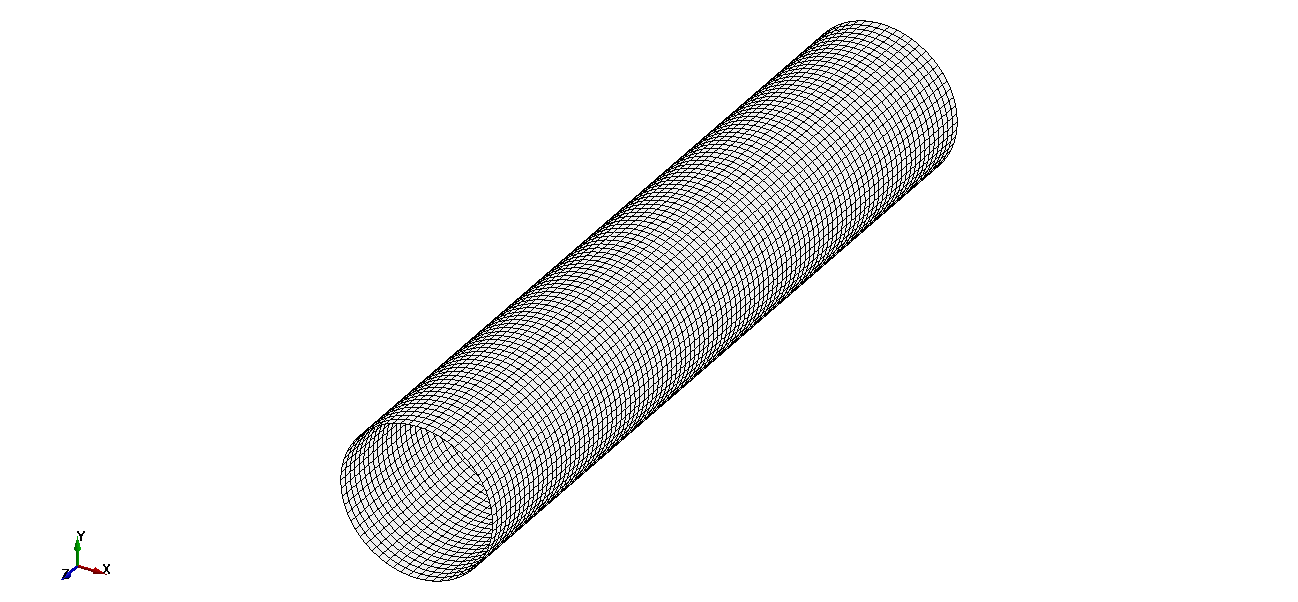
\includegraphics[width=0.5\textwidth]{src/ch3/mesh_perno.png}
\caption{Mallado del perno formador}
\label{fig:mesh_perno}
\end{figure}


% Condiciones de frontera ==================================================================
\subsubsection{Condiciones de frontera}

La descripción de las condiciones de frontera de la sección \ref{sec:condiciones-fronteras} es 
válido también para el análisis tridimensional.

% ==================================== CONTACTOS ============================================
\subsubsection{Contactos}

En la definición de contactos se utilizó un tipo de contacto superficie a superficie
general (\texttt{STS}). El programa de simulación utiliza los coeficientes de fricción 
estático ($FS$) y dinámico ($FD$) para la formulación del coeficiente friccional ($\mu_c$),
que viene dado por la ecuación :

\begin{equation}
\mu_c = FD + (FS - FD) e^{-DCv_{rel}}
\label{eq:frictional_coeff}
\end{equation}

Donde $DC$ es el coeficiente de decaimiento exponencial y $v_{rel}$ la velocidad relativa
entre las superficies en contacto ~\cite{lsdyna-manual}. Los valores del coeficiente de 
fricción estáticoy dinámico se establecieron en 0.2 y 0.1, respectivamente. ~\cite{carvill1993} \\

En la simulación del segundo paso se utilizó el contacto de tipo Single Surface (SS) para 
tomar en cuenta el contacto del blank con él mismo (cerrado del tubo) ~\cite{lsdyna-manual}, 
utilizandotambién los parámetros de fricción indicados anteriormente.

\section{Análisis experimental}

Para validar los resultados obtenidos mediante la simulación por elemento finito, se realizó 
un análisis experimental de esfuerzos y deformaciones mediante la técnica de extensometría. 
De manera general, se instrumentaron cuatro probetas y se sometieron al proceso de formado 
mediante el troquel formador utilizado en producción. En las subsecciones posteriores se describe 
de manera detallada la instrumentación y la realización de las pruebas.

\subsection{Instrumentación de las probetas}

Para llevar a cabo un análisis experimental mediante extensometría primero se hace necesario 
seleccionar la galga extensométrica a utilizar, que dependerá del tipo de fenómeno o proceso 
objeto de estudio. En este caso se seleccionó una galga del tipo \texttt{EP-40-125TQ-350}, la 
cual pertenece a la serie EP, que se utiliza para mediciones de grandes deformaciones posteriores 
a la fluencia ~\cite{vishay-catalog}. Esta galga tiene dimensiones de 0.125 pulgadas por lado, referidas a toda la 
matriz o placa que contiene a la rejilla. La \texttt{EP-40-125TQ-350} es una galga de dos 
elementos a 90° como se muestra en el esquema de la figura \ref{fig:strain_gage}, con 
una resistencia eléctrica de 350 $\Omega$ para cada una. En la tabla \ref{tab:strain_gage_props} 
se resumen las características de importancia de la galga seleccionada.

\begin{center}
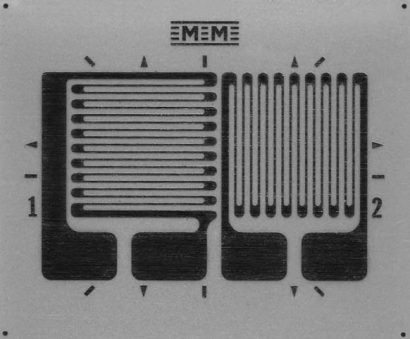
\includegraphics[width=0.35\textwidth]{src/ch3/strain_gage.png}
\captionof{figure}{Esquema de la galga \texttt{EP-40-125TQ-350} utilizada}
\label{fig:strain_gage}
\end{center}

% Tabla de características de la galga
\begin{table}[h]
\centering
\caption{Características de la galga extensométrica \texttt{EP-40-125TQ-350}}
\label{tab:strain_gage_props}
\begin{tabular}{p{6cm} p{4cm}} \hline
Característica & Descripción \\
\hline
Serie & \texttt{EP-40-125TQ-350} \\
Dimensiones & 0.125x0.125 in \\
Resistencia eléctrica &  350 $\Omega$  \\
Factor de galga & 2.04 \\
Rango de deformaciones & $\pm$ 20\% \\
\hline
\end{tabular}
\end{table}

Como se menciona en el párrafo anterior, la \texttt{EP-40-125TQ-350} es una roseta 
a 90° de dos componentes, entonces, se decidió hacer una configuración de 
medio puente de Wheatstone para la lectura de las deformaciones, como se muestra 
en el esquema de la figura \ref{fig:circuito_conexion}, con una de las resistencias 
actuando como una galga pasiva ($R_3$) para el completado del circuito. En la figura 
\ref{fig:diagrama_conexion} se muestra un esquema más aproximado a la conexión real 
realizada, donde se observa que la galga que mide las deformaciones en dirección 
transversal ($R_4$) es la activa y de la cual se tomaron las mediciones. Las deformaciones  
se midieron en esa dirección puesto que es en donde se encuentra la deformación 
principal, lo cual se puede determinar de manera intuitiva debido a que es la dirección 
en la cual se realiza el doblado, además se corrobora mediante los resultados obtenidos 
con el análisis por elementos finitos realizado, del cual se muestra la dirección 
principal de uno de los elementos sobre el eje de doblado en la figura \ref{fig:dir_prin_strain}.


\begin{center}
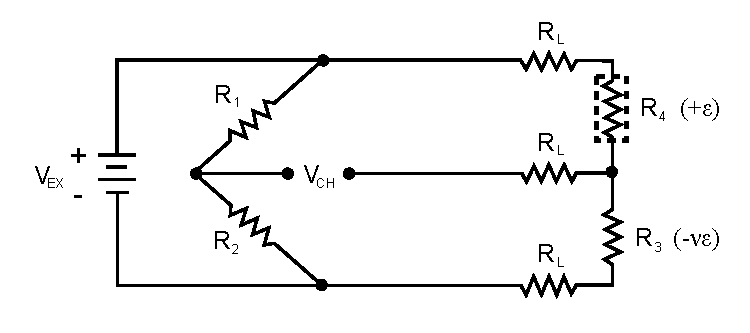
\includegraphics[width=0.65\textwidth]{src/ch3/circuito_conexion.pdf}
\captionof{figure}{Circuito eléctrico de la configuración de medio puente}
\label{fig:circuito_conexion}
\end{center}

\begin{center}
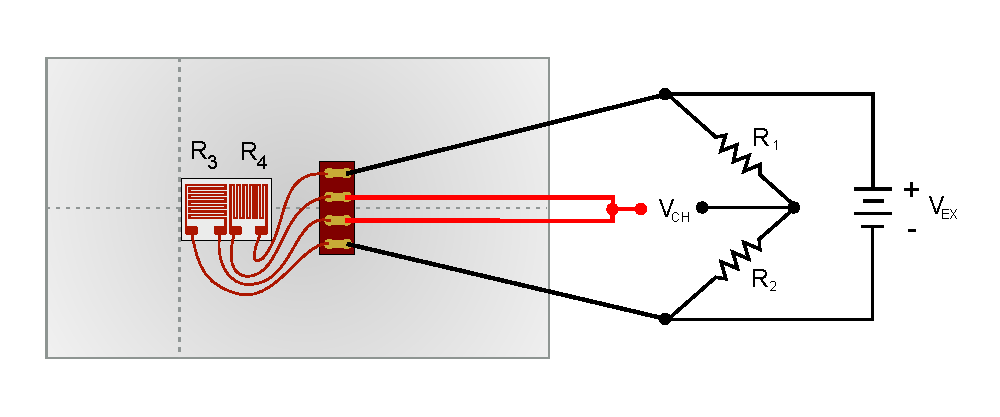
\includegraphics[width=0.65\textwidth]{src/ch3/diagrama_conexion.pdf}
\captionof{figure}{Esquema de la conexión de medio puente realizada}
\label{fig:diagrama_conexion}
\end{center}

En la figura \ref{fig:metodologia_instrumentacion} se muestra la metodología aplicada 
en la instrumentación de cada una de las probetas. Se tuvo especial cuidado con el 
manejo de la galga puesto que ejecutar de manera incorrecta las operaciones necesarias 
para la instrumentación puede dañar la funcionalidad. \\

\begin{center}
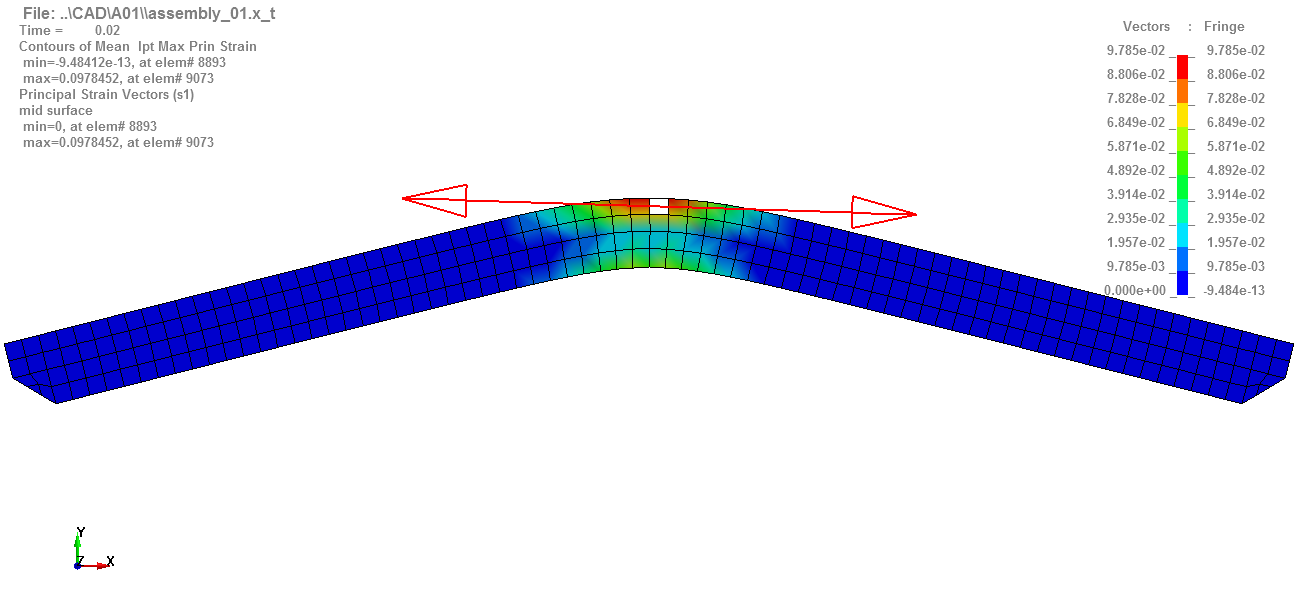
\includegraphics[width=0.65\textwidth]{src/ch3/dir_prin_strain.png}
\captionof{figure}{Dirección de la deformación principal en el \textit{blank}}
\label{fig:dir_prin_strain}
\end{center}

Una vez se tuvieron las probetas se procedió a preparar la superficie de la región en 
la cual se colocó la galga, mediante el uso de lijas y un acondicionador especial 
para lograr una superficie libre de grietas o pequeñas protuberancias, que permita 
una adherencia adecuada de la galga. Evidentemente se utilizaron lijas de diversos 
tamaños de grano en orden descendente para obtener la superficie requerida.\\

\begin{center}
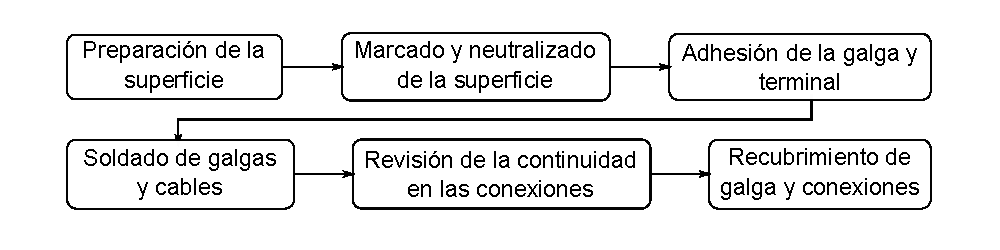
\includegraphics[width=0.95\textwidth]{src/ch3/metodologia_instrumentacion.pdf}
\captionof{figure}{Metodología de la instrumentación}
\label{fig:metodologia_instrumentacion}
\end{center}

Con la superficie preparada se trazaron dos líneas con un lápiz, dispuestas de manera perpendicular 
como se muestra en el esquema de la figura \ref{fig:diagrama_conexion}, una centrada en 
la dirección axial y la otra a 25 mm de uno de los extremos. Luego del marcado de líneas 
se removió el grafito utilizando un cotonete impregnado con líquido neutralizador, deslizándolo en 
dirección de cada una de las líneas trazadas, repitiendo esta operación hasta apreciar que 
el cotonete estuviese libre de residuos de grafito. \\

% \begin{center}
% 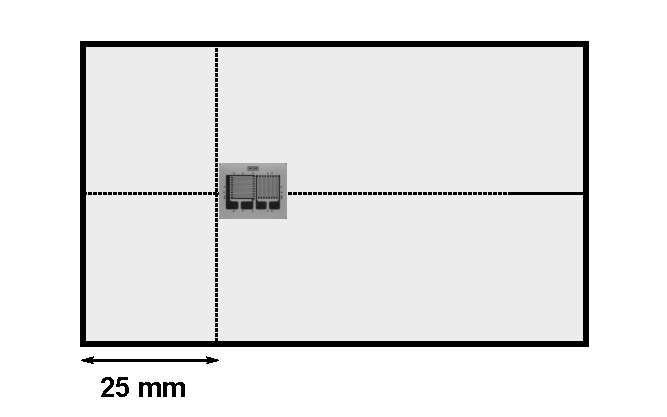
\includegraphics[width=0.65\textwidth]{src/ch3/lineas_galgas.pdf}
% \captionof{figure}{Diagrama del marcado de lineas en la probeta}
% \label{fig:lineas_galgas}
% \end{center}

Con la superficie libre de residuos y grafito se procedió al pegado de la galga, para lo cual 
primeramente se retiró la galga de su empaque, utilizando una pinza pequeña previamente neutralizada, 
y se colocó sobre un cristal neutralizado, luego se procedió a colocar una cinta adhesiva sobre la 
galga de modo que esta se adhiera. Enseguida se procedió a despegar la cinta adhesiva del cristal  
como se muestra en la figura \ref{fig:despegado_vidrio}.

\begin{center}
\includegraphics[width=0.5\textwidth]{src/ch3/despegado_vidrio.png}
\captionof{figure}{Despegado de la galga/cinta del cristal}
\label{fig:despegado_vidrio}
\end{center}

Posteriormente, la cinta/galga se pegó en la probeta, con ayuda de las líneas que fueron trazadas previamente 
para la correcta orientación y ubicación de la galga. Una vez ha sido correctamente ubicada se despegó una porción 
de la cinta que permitiera la aplicación del catalizador y adhesivo en la galga. Se aplicó el catalizador 
de la forma que se observa en el esquema de la figura \ref{fig:aplicacion_catalizador}, el catalizador permite 
que el adhesivo trabaje de manera rápida y fiable. Después de la aplicación del catalizador se dejó 
\textit{reposar} alrededor de 1 minuto para permitir el secado, luego se procedió a la aplicación del 
adhesivo (ver figura \ref{fig:aplicacion_adhesivo}), colocando una gota de este en la región a pegar.\\

Una vez se aplicó el adhesivo se pegó nuevamente la cinta con ayuda de una gasa y mediante un deslizamiento firme 
como se muestra en el esquema de la figura \ref{fig:deslizar_adhesivo}. Se esperó alrededor 
de dos minutos para proceder al despegado de la cinta, el cual debe hacerse con en dirección opuesta 
o un ángulo de 180°.

\begin{center}
\includegraphics[width=0.5\textwidth]{src/ch3/aplicacion_catalizador.png}
\captionof{figure}{Aplicación del catalizador}
\label{fig:aplicacion_catalizador}
\end{center}

\begin{center}
\includegraphics[width=0.5\textwidth]{src/ch3/aplicacion_adhesivo.png}
\captionof{figure}{Aplicación del adhesivo}
\label{fig:aplicacion_adhesivo}
\end{center}

Con las galgas y terminales adheridas a las probetas se procedió al soldado de las diversas conexiones, lo 
cual se realizó mediante un procedimiento convencional de soldadura con estaño.

\begin{center}
\includegraphics[width=0.5\textwidth]{src/ch3/deslizar_adhesivo.png}
\captionof{figure}{Pegado de la galga}
\label{fig:deslizar_adhesivo}
\end{center}

Cuando se tuvieron soldadas las conexiones se procedió a revisar la continuidad con ayuda de un 
multímetro, corrigiendo/resoldando en los casos necesarios. Posteriormente se utilizó un lector 
de deformaciones (P3) ~\cite{p3indicator} para conectar y realizar lecturas para verificar la funcionalidad de las 
galgas extensométricas.\\

Después de realizar las pruebas y verificaciones anteriores se recubrieron las zonas de instalación 
de galga de cada probeta mediante una resina adecuada para estas tareas, con la finalidad de 
proteger las galgas y conexiones. Las probetas ya instrumentadas se muestran en la 
figura \ref{fig:probetas_instrumentadas}.

\begin{center}
\includegraphics[width=0.65\textwidth]{src/ch3/probetas_instrumentadas.jpg}
\captionof{figure}{Probetas instrumentadas}
\label{fig:probetas_instrumentadas}
\end{center}


\subsection{Realización de las pruebas}

TODO




